\documentclass[a4paper,12pt]{article}

\usepackage[utf8]{inputenc}
\usepackage[T1]{polski}
\usepackage{helvet}
\usepackage{graphicx}
\usepackage{color}
\usepackage{geometry}
\usepackage{cite}
\usepackage{url}

\geometry{hmargin={2cm, 2cm}, height=10.0in}
%\includeonly{introduction}

\begin{document}


\thispagestyle{empty}
%% ------------------------ NAGLOWEK STRONY ---------------------------------

\includegraphics[height=37.5mm]{../images/agh_nzw_a_pl_1w_wbr_rgb_150ppi.jpg}\\
\rule{30mm}{0pt}
{\large \textsf{Wydział Fizyki i Informatyki Stosowanej}}\\
\rule{\textwidth}{3pt}\\
\rule[2ex]
{\textwidth}{1pt}\\
\vspace{7ex}
\begin{center}
{\LARGE \bf \textsf{Praca magisterska}}\\
\vspace{13ex}
% --------------------------- IMIE I NAZWISKO -------------------------------
{\bf \Large \textsf{Łukasz Hanusiak}}\\
\vspace{3ex}
{\sf\small kierunek studiów:} {\bf\small \textsf{informatyka stosowana}}\\
\vspace{1.5ex}
{\sf\small specjalność:} {\bf\small \textsf{informatyka w nauce i technice}}\\
\vspace{10ex}
%% ------------------------ TYTUL PRACY --------------------------------------
{\bf \huge \textsf{Rozwój platformy robota mobilnego}}\\
\vspace{14ex}
%% ------------------------ OPIEKUN PRACY ------------------------------------
{\Large Opiekun: \bf \textsf{dr hab. inż. Marek Idzik}}\\
\vspace{22ex}
{\large \bf \textsf{Kraków, czerwiec 2010}}
\end{center}
%% =====  STRONA TYTUŁOWA PRACY MAGISTERSKIEJKIEJ ====

\newpage

%% =====  TYŁ STRONY TYTUŁOWEJ PRACY MAGISTERSKIEJKIEJ ====
{\sf Oświadczam, świadomy(-a) odpowiedzialności karnej za poświadczenie nieprawdy, że niniejszą pracę dyplomową wykonałem(-am) osobiście i samodzielnie i  nie korzystałem(-am) ze źródeł innych niż wymienione w pracy.}

\vspace{14ex}

\begin{center}
\begin{tabular}{lr}
~~~~~~~~~~~~~~~~~~~~~~~~~~~~~~~~~~~~~~~~~~~~~~~~~~~~~~~~~~~~~~~~~ &
................................................................. \\
~ & {\sf (czytelny podpis)}\\
\end{tabular}
\end{center}

%% =====  TYL STRONY TYTULOWEJ PRACY MAGISTERSKIEJKIEJ ====

\newpage
\rightline{Kraków, ?? czerwca 2010}
\begin{center}
{\bf Tematyka pracy magisterskiej i praktyki dyplomowej
Łukasza Hanusiaka,
studenta V roku studiów kierunku informatyka stosowana, informatyka w nauce i technice}\\
\end{center}

Temat pracy magisterskiej:
{\bf Rozwój platformy robota mobilnego}\\

\begin{tabular}{rl}

Opiekun pracy:                  & dr hab. inż. Marek Idzik\\
Recenzenci pracy:               & ??? ??? \\
Miejsce praktyki dyplomowej:    & WFiIS AGH, Kraków\\
\end{tabular}

\begin{center}
{\bf Program pracy magisterskiej i praktyki dyplomowej}
\end{center}

\begin{enumerate}
\item Omówienie realizacji pracy magisterskiej z opiekunem.
\item Zebranie i opracowanie literatury dotyczącej tematu pracy.
\item Praktyka dyplomowa:
\begin{itemize}
\item zapoznanie się z ideą...,
\item uczestnictwo w eksperymentach/przygotwanie oprogramowania...,
\item dyskusja i analiza wyników...
\item sporządzenie sprawozdania z praktyki.
\end{itemize}
\item Kontynuacja obliczeń związanych z tematem pracy magisterskiej.
\item Zebranie i opracowanie wyników obliczeń.
\item Analiza wyników obliczeń numerycznych, ich omówienie i zatwierdzenie przez opiekuna.
\item Opracowanie redakcyjne pracy.
\end{enumerate}


\noindent
Termin oddania w dziekanacie: ?? czerwca 2010\\[1cm]

\begin{center}
\begin{tabular}{lcr}
.............................................................. & ~~~ &
.............................................................. \\
(podpis kierownika katedry) & & (podpis opiekuna) \\
\end{tabular}
\end{center}

\newpage

\noindent
Na kolejnych dwóch stronach proszę dołączyć kolejno recenzje pracy popełnione przez Opiekuna oraz Recenzenta (wydrukowane z systemu MISIO i podpisane przez odpowiednio Opiekuna i Recenzenta pracy). Papierową wersję pracy (zawierającą podpisane recenzje) proszę złożyć w dziekanacie celem rejestracji co najmniej na tydzień przed planowaną obroną.

\linespread{1.3}
\selectfont

\newpage
\tableofcontents

\newpage
\part{Wstęp teoretyczny}
Celem pracy magisterskiej jest rozwój systemu robota mobilnego
zrealizowanego pierwotnie w pracy magisterskiej pt.: ,,Rozwój systemu sterowania
dla robota mobilnego''\cite{KmakMScThesis2009}. Temat pracy daje dużą swobodę w
wyborze kierunku rozwoju części sprzętowej oraz programowej robota. Niniejsza
praca zajmuje się proces rozbudową robota Dark Explorer, począwszy od analizy
konfiguracji początkowej, poprzez poprawę wydajności istniejących elementów, aż
po dodanie całkiem nowych funkcjonalności. Praca magisterska wymagała wiedzy z
zakresu elektroniki, fizyki oraz szeroko pojętej informatyki.

W ramach pracy magisterskiej zostały podłączone oraz oprogramowane czujniki
składające się na inercjalną jednostkę pomiarową. Jednostka ta umożliwia
rejestrowanie toru ruchu, po którym robot jest przenoszony przez użytkownika.
Podjęto również próbę stworzenia inercjalnego systemu nawigacyjnego w celu
rozwiązania problemu rekonstrukcji ścieżki powrotnej na podstawie danych
zarejestrowanych przy pomocy czujnika przyspieszenia oraz żyroskopu. W trakcie
odtwarzania powrotnego toru ruchu robot, wykorzystując dane z dołączonych do
niego dalmierzy, jest w stanie uniknąć zderzenia z napotkanymi przeszkodami
jednocześnie starając się dotrzeć do punktu startowego. W pracy magisterskiej
zawarty jest również przewodnik pozwalający programistom, nie posiadającym
doświadczenia w tworzeniu oprogramowania dla systemów wbudowanych, zaznajomić się
z narzędziami pomocnymi w rozwoju programów sterujących mikrokontrolerami
opartymi o architekturę ARM. Poruszono także tematykę rozwoju aplikacji
sterujących robotem dedykowanych na urządzenia mobilne oraz stacjonarne. Efektem
tego jest stworzone oprogramowanie działające na komputerach oraz telefonach z
obsługą technologii Java ME oraz .NET. Podczas tworzenia oprogramowania położono
szczególny nacisk na przenośność wszystkich rozwiązań na różne środowiska
uruchomieniowe oraz intuicyjną obsługę i prostą rozbudowę oprogramowania.

W rozdziale pierwszym przedstawiono dzieje robotyki od jej początków, aż po dzień
dzisiejszy. W ramach tego rozdziału, zaprezentowane zostały dziedziny w jakich
współcześnie roboty znajdują zastosowanie. Nie zabrakło również podstawowych
informacji na temat sposobów klasyfikacji i podziału robotów. Rozdział ten ma na
celu wprowadzenie użytkownika w zagadnienia z którymi robotyka zmaga się na co
dzień.

Rozdział drugi przedstawia analizę sprzętu oraz oprogramowania robota Dark
Explorer stworzonych w ramach poprzedniej pracy magisterskiej. Zwraca on uwagę na
możliwości oraz potencjalne przeszkody które mogą się pojawić podczas rozwoju
robota.

Trzeci rozdział opisuje narzędzia, oraz sposób ich konfiguracji, niezbędne
podczas rozwoju oprogramowania dla systemów wbudowanych. Ze względu na znaczące
różnice pomiędzy narzędziami przeznaczonymi dla systemu Windows i Linux, zostały
one omówione w ramach oddzielnych podrozdziałów.

W rozdziale czwartym poruszana jest tematyka związana z tworzeniem oprogramowania
sterującego robotem działającego na urządzeniach mobilnych oraz stacjonarnych.

Rozdział piąty przedstawia rozszerzenia warstwy sprzętowej wprowadzone w trakcie
realizacji pracy magisterskiej. Czytelnik znajdzie tutaj szczegółowy opis zasady
działania i możliwych zastosowań dla czujników dołączonych do nowej wersji robota
Dark Explorer. W ramach rozdziału omówiono również sposób konstrukcji obudowy
pozwalającej na wygodne podłączanie wszystkich elementów rozszerzających
dotychczasowe możliwości robota.

Szósty rozdział prezentuje funkcje oprogramowania systemu wbudowanego
rozwiązujące problemy takie jak: rekonstrukcja ścieżki powrotnej, omijanie
przeszkód, pobieranie obrazu z kamery z maksymalną dostępną rozdzielczością oraz
detekcja twarzy na obrazie statycznym. Opisany jest również protokół komunikacji
bluetooth warstwy aplikacji modelu referencyjnego ISO.

Złożoność problemów realizowanych w ramach tej pracy magisterskiej oraz szeroki
zakres wiedzy konieczny do jej realizacji wymagał aby była ona realizowana w
zespole dwuosobowym.
\section{Historia i rozwój robotyki}
Robotyka jest stosunkowo młodą dziedziną nauki łączącą różne gałęzie nauk
technicznych i nie tylko. Do pełnego zrozumienia zagadnień współczesnej robotyki
oraz budowy i zastosowań robotów konieczna jest niejednokrotnie rozległa wiedza
na temat elektroniki, mechaniki, inżynierii przemysłowej, matematyki oraz
szeroko pojętej informatyki. Ponadto wiele nowopowstałych gałęzi wiedzy
zajmujących się rozwojem sztucznej inteligencji, modelowaniem sztucznego życia czy rozwojem
inżynierii wiedzy coraz częściej staje się nierozerwalnie związane z problemami
współczesnej robotyki. Nie należy zapominać również o tym, że rozwój inżynierii
wytwarzania oraz automatyki przemysłowej pozwala na nieustanny rozwój robotyki z
którą mamy do czynienia w przemyśle w dniu dzisiejszym.\\
\\
Pojęcie ``Robot'' w literaturze pojawił się po raz pierwszy w sztuce czeskiego
pisarza Karel'a Capka w roku 1920. Termin ``robot'' oznacza w języku czeskim
pracę lub służbę przymusową. Nieco ponad 20 lat później, amerykański uczony i
pisarz Isaac Assimov w jednym ze swoich opowiadań po raz pierwszy używa słowa
robotyka. W kolejnych latach Assimov w swojej twórczości niejednokrotnie wraca
do problemu robotyki skutkiem czego jest wydanie w 1950 roku zbioru opowiadań
pod tytułem ``Ja, robot''. Jako ciekawostkę można dodać, że w wydanym w 1942
roku opowiadaniu pod tytułem ``Zabawa w berka'', Assimove wprowadza trzy prawa
robotyki, według których zdaniem autora powinny być programowane roboty.
\begin{description}
\item[Prawo pierwsze] \hfill \\
Robot nie może zranić istoty ludzkiej, ani przez zaniedbanie narazić człowieka
na zranienie. 
\item[Prawo drugie] \hfill \\
Robot musi spełniać polecenia wydawane przez człowieka, poza poleceniami
sprzecznymi z prawem pierwszym.
\item[Prawo trzecie] \hfill \\
Robot musi chronić samego siebie dopóki nie jest to sprzeczne z prawami
pierwszym i drugim.
\end{description} 
Nieco później, Isaac Assimov, jako uzupełnienie i prawo nadrzędne dodaje prawo
zerowe o następującym brzmieniu ``Robot nie może szkodzić ludzkości, ani przez zaniedbanie narazić ludzkości na
szkodę''. Oprócz wspomnianych powyżej podstawowych praw, zdefiniowano również
inne prawa wynikające z prowadzonych badań w tej dziedzinie i rozwoju robotyki.\\
\\
Dzięki gwałtownemu rozwojowi techniki w czasie II wojny światowej w roku 1956
GC. Devol i JF. Engelberger zainspirowani twórczością Assimov'a zaprojektowali i
stworzyli pierwszy w dziejach ludzkości działający egzemplarz robota.
Engelberger założył firmę pod nazwą ``Unimation'' zajmującą się automatyzacją,
pierwszym robotem stworzonym przez firmę Engelbergera był robot nazwany
``Unimate''. Został on zainstalowany w fabryce General Motors w Trenton gdzie
został przystosowany do obsługi wysokociśnieniowej maszyny odlewniczej. W
kolejnych latach roboty firmy ``Unimation'' znalazły swoje zastosowanie w innych
gałęziach przemysłu, a sam Engelberger otrzymał miano ojca robotyki.\\
\\
Nieco później, bo w roku 1979 Robotics Industries Association 
zdefiniowało robota jako wielofunkcyjny, programowalny manipulator
zaprojektowany do przenoszenia materiałów, narzędzi, części urządzeń poprzez
serię programowalnych ruchów wykonywanych w celu realizacji różnych zadań.
W myśl wspomnianej definicji jedną z podstawowych cech robota jest jego
progrmowalność i możliwość dostosowywania się do zmiennych warunków środowiska
pracy. \\
Pierwsze roboty projektowano z myślą o zastosowaniu ich do realizacji
elementarnych zadań związanych z przenoszeniem elementów z jednego punktu do
drugiego. Program pracy robota miał więc charakter sekewencji operacji
prowadzących do realizacji określonego przez programistę zadania. W miarę
rozwoju technicznego, stawiane przed robotami zadania wymusiły użycie przez
konstruktorów czujników które pozwalały na zwiększenie poziomu interakcji
robotów z otoczeniem, a co za tym idzie umożliwiły realizowanie zadań o wysokim
stopniu złożoności. Od tego momentu kierunek rozwoju robotyki obrał
sobie za cel stworzenie maszyny na tyle uniwersalnej i niezależnej aby mogła
nosić miano androida. Jednak do realizacji tego zadania konieczne jest
opracowanie sztucznej inteligencji na którą z pewnością przyjdzie nam jeszcze
trochę poczekać. \\
\\
Pierwszym krokiem na drodze do stworzenia androida było oderwanie robota od
stałego miejsca instalacji i pozwolenie mu w miarę możliwości swobodne
poruszanie się dostępnej mu przestrzeni roboczej. Tak powstała klasa robotów
które mogą przemieszczać się za pomocą kół, gąsienic czy nawet kończyn lub
odnóży. Roboty tego typu potrafią pływać, latać i sprawnie poruszać się
po lądzie dodatkowym ich atutem jest fakt iż większość z nich posiada niemal
całkowitą autonomię i ograniczona jest jedynie poprzez wielkość otoczenia w
jakim zostały umieszczone. Takim sposobem roboty powstała grupa robotów
nazywanych robotami mobilnymi. Cechą wspólną wszystkich urządzeń z tej rodziny
była umiejętność swobodnego przemieszczania się oraz analiza najbliższego
otoczenia. Na tej podstawie maszyna mogła przeprowadzić wnioskowanie pozwalające
na podejmowanie dalszych akcji czy też zakomunikowanie użytkownikowi odczytanych
parametrów środowiska.\newpage
Historię robotów mobilny zapoczątkował amerykański Uniwersytet w Stanford gdyż
w roku 1968 jako pierwszy stworzył w pełni działający model robota mobilnego pod
nazwą Shakey. Nazwa została zainspirowana szarpanymi ruchami z jakimi robot się
poruszał. Głównym zadaniem robota było modelowanie otoczenia w którym się
znajdował. W ślad za Uniwersytetem w Stanford ruszyło MIT. W roku 1983 posiadali
już pierwszy działający model robota swobodnie skaczącego. Niecałe 6
lat później MIT stworzyło pierwszego robota kroczącego wzorowanego na owadach.
Robot ten sterowany był za pomocą wielowarstwowych automatów o stanach
skończonych, a ze światem zewnętrznym komunikował się za pomocą czułek,
inklinometrów, czujników zbliżeniowych na podczerwień. Genghis, bo tak
nazwany został robot, posiadał na pokładzie 4 ośmiobitowe jednostki obliczeniowe, ważył
niecały kilogram i miał 35 cm długości.

\begin{figure}[hb]
 \centering
 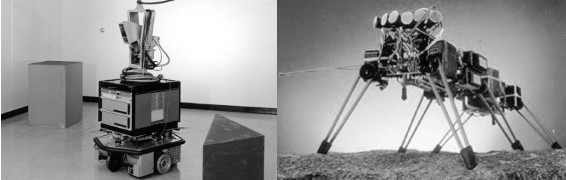
\includegraphics[height=50mm]{../images/ch01/shakey_and_genghis.png}
 \caption{Od lewej: Shakey (Stanford), Genghis (MIT) }
 \label{fig:RobotsHistory_Shakey_Genghis}
\end{figure}

Po sukcesie wspomnianych projektów,
rozwój robotów mobilnych następował już bardzo dynamiczne. W latach 90
powstawało wiele różnych modeli robotów o bardzo różnorodnych rodzajach napędów
oraz zestawach czujników umożliwiających interakcje ze światem zewnętrznym.

\begin{figure}[hb]
 \centering
 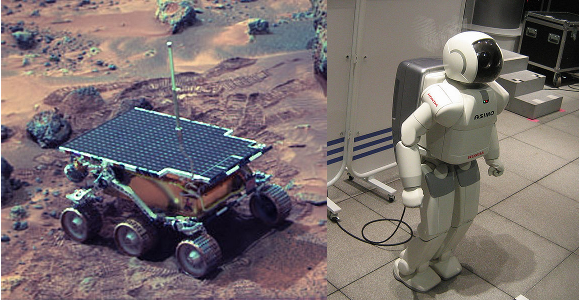
\includegraphics[height=60mm]{../images/ch01/pathfinder_and_asimo.png}
 \caption{Kolejno: Pathfinder (NASA), Asimo (Honda)}
 \label{fig:RobotsHistory_Pathfinder_Asimo}
\end{figure}

Swoistym ukoronowaniem prac było w 1997 roku stworzenie przez NASA robota o
nazwie Pathfinder. Robot wyposażony był w czujniki laserowe, stereowizję,
żyroskopy i inne rodzaje czujników o charakterze badawczym. Zasilany był on
bateriami słonecznymi które pozwoliły mu na 83 dni nieprzerwanej pracy podczas
której robot przebyło około 100 metrów i wykonał 230 manewrów. W ostatnich
latach do największych osiągnięć robotyki mobilnej można z pewnością zaliczyć
powstanie robotów humanoidalnych takich jak japoński ASIMO. Robot ten ważył 54
kg i posiadał 130 cm wysokości. Wersja z roku 2005 potrafiła biegnąc osiągnąć
prędkość dochodzącą nawet do do 6 km/h. Ponad to robot potrafił wchodzić w
interakcję z otoczającymi go ludźmi i przedmiotami. Urządzenie stworzone przez
inżynierów z firmy Honda potrafiło rozpoznawać gesty takie jak podanie ręki,
wskazanie kierunku czy machanie ręką na porzegnanie. Robot równie dobrze radził
sobie z rozpoznawaniem twarzy, dźwięków i analizą otaczającego go środowiska.
Potrafił on rozpoznać i omijać niebezpieczeństwa postawione na jego drodze jak
na przykład schody czy osoby poruszające się w jego kierunku.\\
\\
Obserwując postęp w dziedzinie robotyki można odnieść wrażenie iż w dzisiejszych
czasach roboty znalazły dla siebie zastosowanie niemal w każdej dziedzinie
życia. Od wielu lat sprawdzają się już w przemyśle, transporcie, budownictwie
oraz są niezastąpione w środowiskach nieprzyjaznych człowiekowi, takich jak
podmorskie głębiny czy otchłań kosmosu. Obszar zastosowań robotów jest
tak szeroki iż wydawać się może, że jedynym czynnikiem ograniczającym rozwój
współczesnej robotyki są względy czysto ekonomiczne. Nie staje to jednak na
przeszkodzie do projektowania i tworzenia przez konstruktorów z całego świata
rozwiązań powoli przybliżających ludzkość do stworzenia w pełni samodzielnego
oraz inteligentnego androida.

\section{Elementy składowe i budowa robotów}
\subsection{Podstawowe układy i zespoły}
\subsection{Układ zasilania}
\subsection{Układ sterowania}
\subsection{Układ ruchu}
\section{Klasyfikacja robotów}
\subsection{Klasyfikacja na podstawie własności geometrycznych}
\subsection{Klasyfikacja na podstawie budowy jednostki kinematycznej}
\subsection{Klasyfikacja ze względu na obszar zastosowań}

\newpage
\part{Dark Explorer pod lupą}
W tym rozdziale zostanie opisana konfiguracja pierwotna robota z wyszczególnieniem elementów, które mogą być problemem przy dalszym rozwoju możliwości tego urządzenia.
\begin{figure}[!ht]
 \centering
 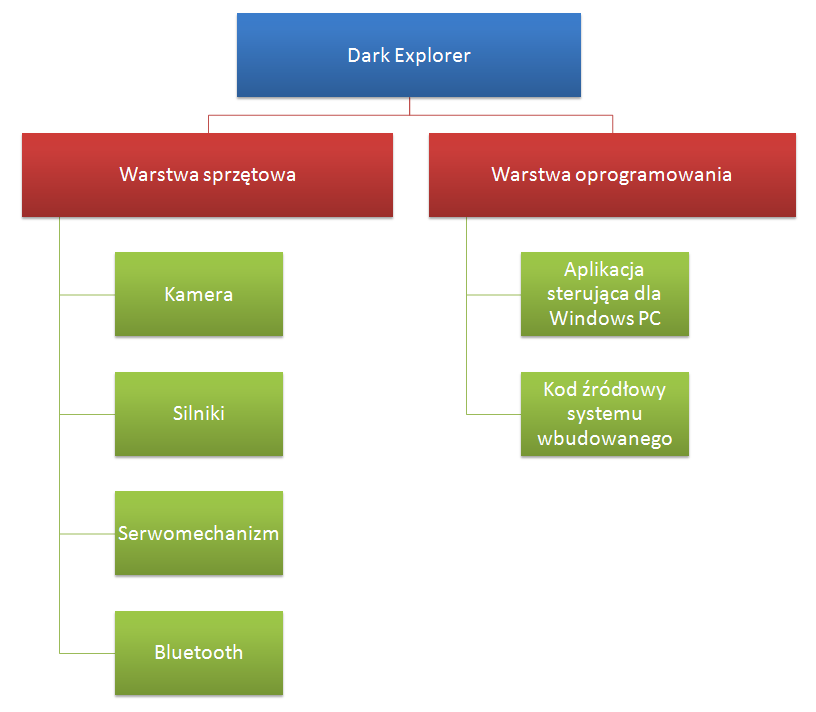
\includegraphics[height=125mm]{../images/ch02/kmak_platform.png}
 \caption{Struktura platformy robota mobilnego zrealizowanej w ramach
 poprzedniej pracy magisterskiej\cite{KmakMScThesis2009}}
 \label{fig:KmakPlatform}
\end{figure}

\section{Analiza sprzętu}
Dark Explorer jest autonomicznym robotem mobilnym z wbudowaną kolorową kamerą cyfrową VGA. Jego podstawowe możliwości to:
\begin{itemize}
 \item jazda ze zmienną prędkością w przód, tył, lewo oraz prawo
 \item komunikacja z urządzeniami zewnętrznymi przy pomocy technologii bluetooth
 \item wykonywanie zdjęć z maksymalną rozdzielczością $160x100$ pikseli w kolorze oraz $320x200$ pikseli w odcieniach szarości
 \item poruszanie wieżyczką na której zainstalowana jest kamera
 \item wykrywanie prostych wzorców przy pomocy analizy obrazu oraz podążanie za nimi
\end{itemize}

\subsection{Elementy elektroniczne}
Dark Explorer został wyposażony w mikrokontroler zarządzający AT91Sam7s256 o częstotliwości pracy zegara maksymalnie do 50 MHz oraz wbudowanej szybkiej pamięci SRAM 64 kB. Mikrokontroler ten jest bogaty w różnego rodzaju urządzenia peryferyjne takie jak na przykład: TWI\footnote{TWI -- Two Wire Interfece znany również jako $I^{2}C$, interfejs szeregowej komunikacji danych}, RTT\footnote{RTT -- Real Time Timer, służy do odmierzania dłuższych odcinków czasu}, PDC\footnote{PDC -- Peripheral DMA Controller, kontroler DMA}, AIC\footnote{AIC -- Advanced Interrupt Controller, kontroler przerywań}, PWM\footnote{PWM -- Pulse Width Modulation Controller}, ADC\footnote{ADC -- Analog to Digital Converter, konwerter analogowo cyfrowy}. To tylko część z nich. Dzięki tak wielkiemu wyborowi urządzeń peryferyjnych mikrokontroler ten daje nam duże możliwości rozwoju konfiguracji. Częstotliwość pracy mikrokontrolera ARM7 jest wystarczająca do zadań przez niego wykonywanych.

Większość elementów elektronicznych robota jest umieszczonych na płycie głównej zaprojektowanej przez autora projektu robota. Jest ona bardzo dobrze przemyślana ponieważ pozwala na wykorzystywanie urządzeń peryferyjnych mikrokontolera w praktycznie dowolny sposób. Większość wyjść oraz wejść mikrokontrolera nie jest połączona na stałe z konkretnymi podzespołami Dark Explorera lecz poprzez zworki, które pozwalają podłączanie i odłączanie poszczególnych urządzeń.

\begin{figure}[!ht]
 \centering
 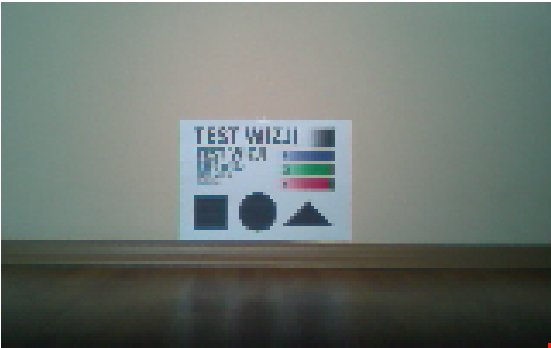
\includegraphics[height=50mm]{../images/ch02/160x100C.jpg}
 \caption{Obraz wykonany przy pomocy kamery zamontowanej w robocie. 160 x 100 pikseli w kolorze. \cite{KmakMScThesis2009}}
 \label{fig:160x100C}
\end{figure}

Twórca Dark Explorera wyposażył go kamerę cyfrową o maksymalnej rozdzielczości $640x480$ pikseli. Jest to urządzenie $PO6040$ firmy Pixelplus. Można go konfigurować przy pomocy interfejsu $I^{2}C$. W konfiguracji pierwotnej robot potrafi odbierać zdjęcia o maksymalnej rozdzielczości $320x200$ pikseli w odcieniach szarości(rys. \ref{fig:320x200BW}) oraz $160x100$ pikseli w kolorze (rys. \ref{fig:160x100C}). Tak niskie rozdzielczości nie są wystarczające do wykrywania i tym bardziej rozpoznawania twarzy na obrazie dlatego też konieczna jest poprawa tych parametrów.

W skład robota wchodzą także silniki napędowe, serwomechanizm, dioda mocy oraz moduł bluetooth. Wszystkie te elementy muszą być podłączone do mikrokontrolera przez konkretne wejścia/wyjścia. Z tego powodu do dyspozycji osób przeprowadzających dalszy rozwój robota pozostało jedynie pięć wejść/wyjść cyfrowych oraz trzy wejścia analogowe. Jest to kolejna przeszkoda którą trzeba będzie pokonać.

\begin{figure}[!ht]
 \centering
 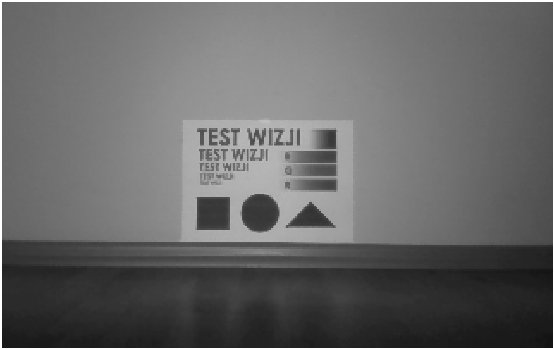
\includegraphics[height=50mm]{../images/ch02/320x200B&W.jpg}
 \caption{Obraz wykonany przy pomocy kamery zamontowanej w robocie. 320 x 200 pikseli w odcieniach szarości \cite{KmakMScThesis2009}}
 \label{fig:320x200BW}
\end{figure}

Robot mobilny komunikuje się z urządzeniami zewnętrznymi przy pomocy modułu bluetooth BTM-222 firmy Rayson. Maksymalna przepustowość danych z jaką potrafi działać wynosi 3Mb/s. Obsługiwane przez niego interfejsy to: USB, UART oraz PCM. Mikrokontroler komunikuje się z modułem bluetooth przy pomocy interfejsu UART o maksymalnej przepustowości 460,8 kb/s. Jak widać takie rozwiązanie nie wykorzystuje pełnych możliwości modułu BTM-222. Bardziej efektywne byłoby skorzystanie z interfejsu USB który potrafi przesyłać dane z prędkością maksymalną od 1,5Mb/s w standardzie USB 1.0 do 5Gb/s w standardzie USB 3.0. Aby dokonać zmiany interfejsu komunikacyjnego pomiędzy mikrokontrolerem a modułem bluetooth konieczna jest ingerencja w konstrukcję płyty głównej robota, gdyż BTM-222 jest przylutowany bezpośrednio do niej \ref{fig:BTM222}.

\begin{figure}[!ht]
 \centering
 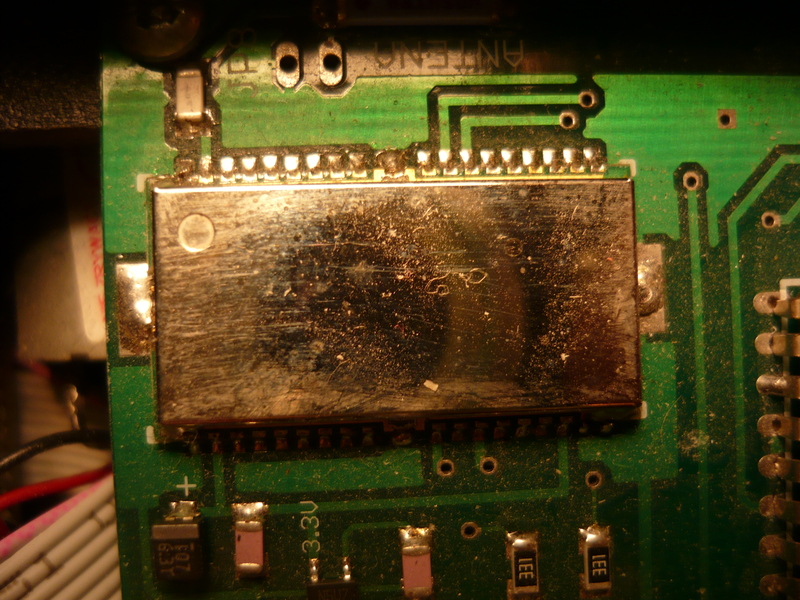
\includegraphics[height=50mm]{../images/ch02/btm-222.jpg}
 \caption{Zdjęcie modułu bluetooth zamontowanego na płycie głównej robota.}
 \label{fig:BTM222}
\end{figure}

\subsection{Elementy mechaniczne}
Konstrukcja obudowy Dark Explorera została wykonana z tworzywa sztucznego i jest dopasowana do elementów które zostały zaprojektowane przez autora. Wewnątrz obudowy nie ma miejsca na jakiekolwiek nowe podzespoły, dlatego też konieczna będzie jej modyfikacja (rys. \ref{fig:KmakMainBoard}).

\begin{figure}[!ht]
 \centering
 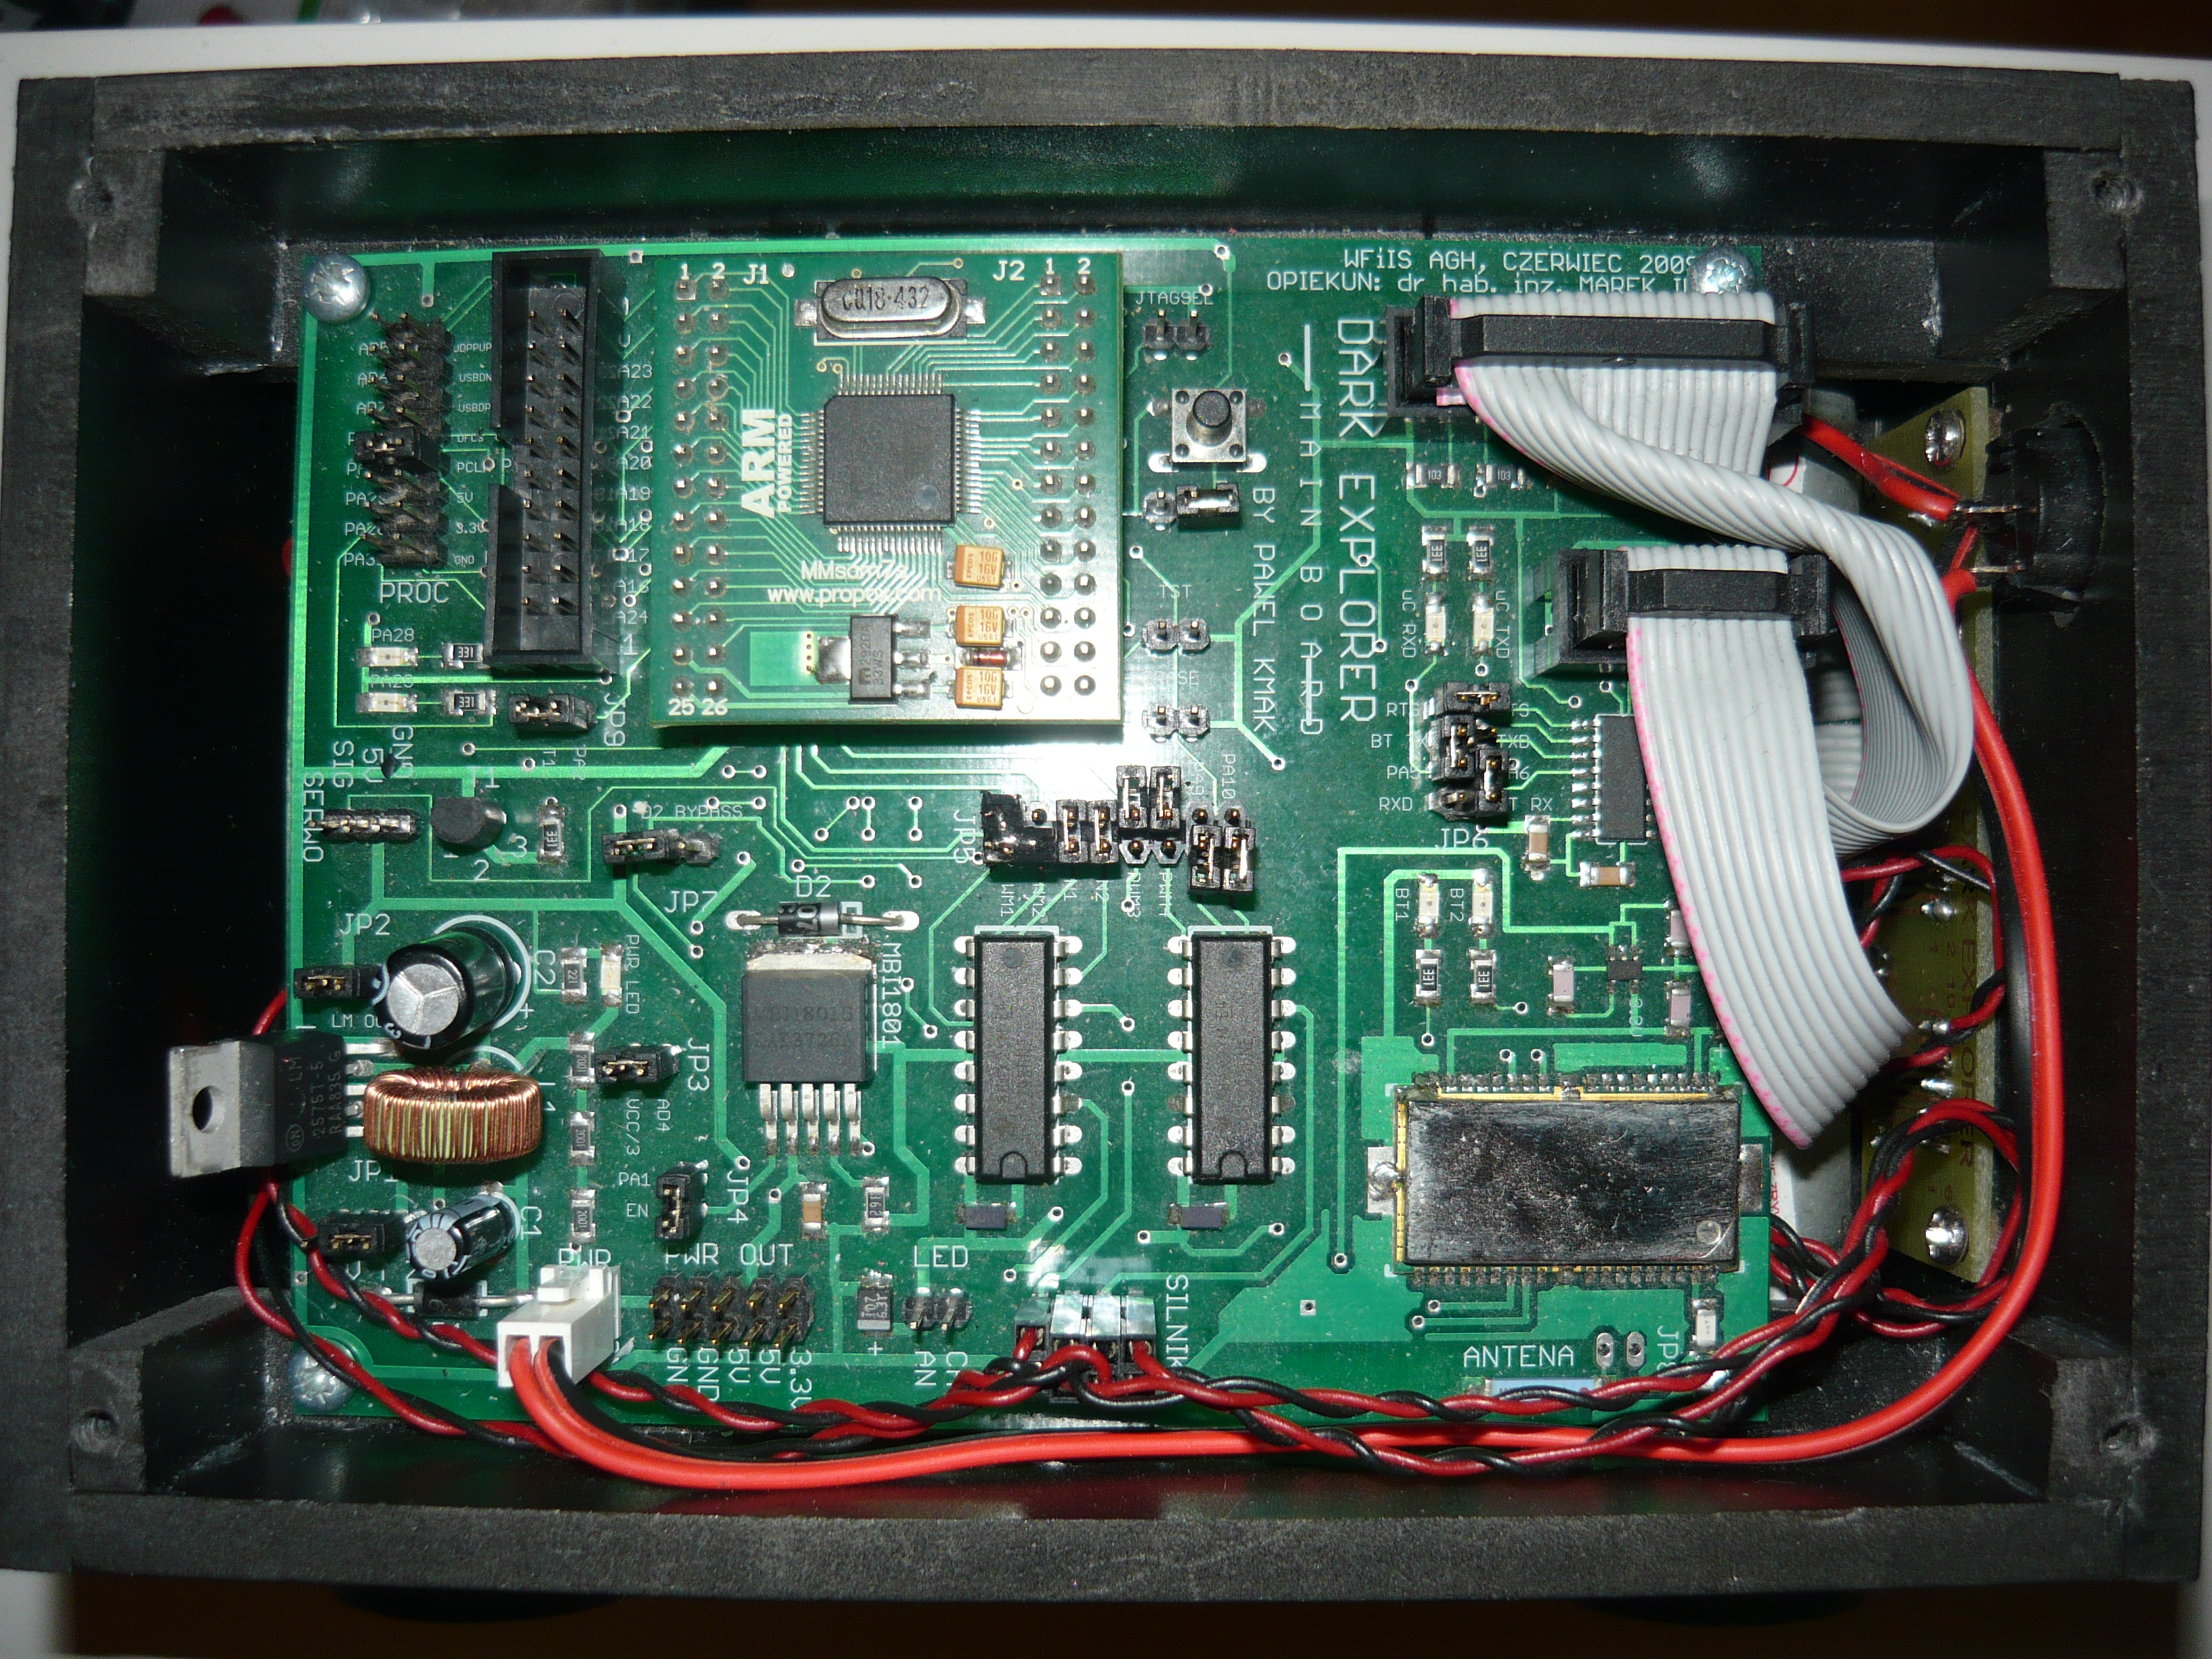
\includegraphics[height=75mm]{../images/ch02/main_board.jpg}
 \caption{Widok na płytę główną Dark Explorer'a}
 \label{fig:KmakMainBoard}
\end{figure}

Podczas testów konfiguracji pierwotnej zauważono lekkie kłopoty robota z poruszaniem się po gładkich powierzchniach. Najprawdopodobniej jest to spowodowane kółkami (rys. \ref{fig:KmakWheel}) zamontowanymi przy robocie, które tracą przyczepność na nieco bardziej śliskim podłożu. Możliwe, że podczas rozwoju robota, konieczna będzie ich wymiana w celu zapewnienia dobrej przyczepności i poprawnego toru jazdy urządzenia.

\begin{figure}[!ht]
 \centering
 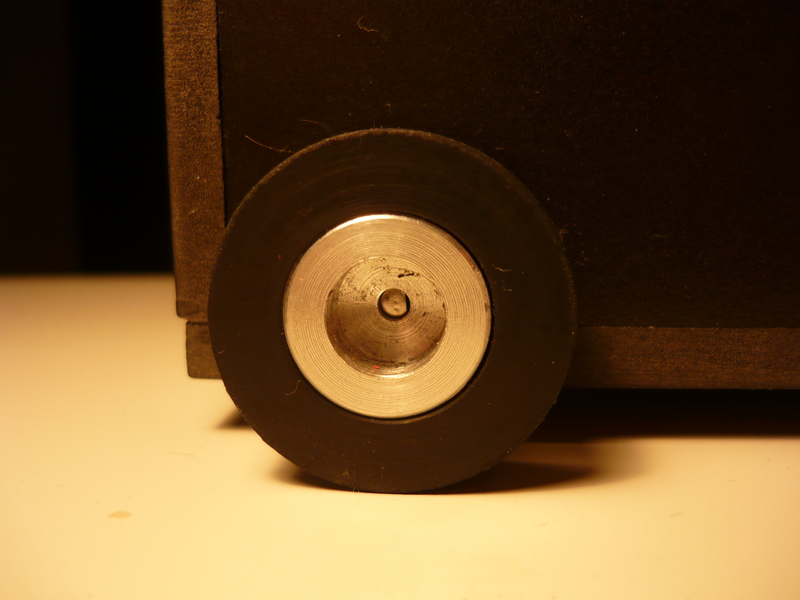
\includegraphics[height=75mm]{../images/ch02/wheel.jpg}
 \caption{Koło napędowe Dark Explorer'a}
 \label{fig:KmakWheel}
\end{figure}

\chapter{Analiza istniejącej platformy software'owej}
\section{Analiza oprogramowania robota - firmware}
\section{Analiza programu sterującego}


\newpage
\part{Platforma do rozwoju oprogramowania}
Podczas przygotowywania się do rozpoczęcia pracy z nową technologią, każdy
programista powinien być świadomy tego jakie są istniejące narzędzia, które mogą
mu pomóc w pracy. W tym rozdziale opisany jest sposób instalacji oraz używania
narzędzi wykorzystywanych przez autorów tej pracy.

\begin{figure}[!ht]
 \centering
 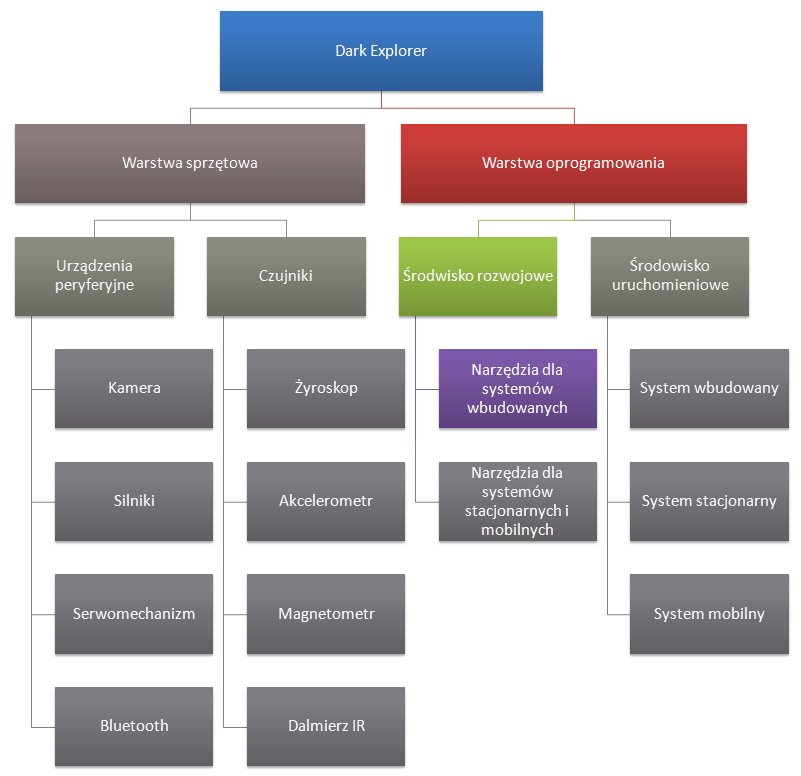
\includegraphics[height=125mm]{../images/ch03/dark_explorer_platform_ide_embeded.png}
 \caption{Struktura platformy robota mobilnego po zakończeniu prac. Kolorem oznaczono zakres prac opisanych w bierzącym rozdziale.}
 \label{fig:DarkExplorerPlatformIDE}
\end{figure}

\section{Narzędzia dla systemu Windows}
\label{sec:embeded-win-tools}
Pierwszym krokiem do przygotowania środowiska rozwojowego umożliwiającego
rozwijanie oprogramowania sterującego robotem jest instalacja sterowników
wymaganych przez system Windows do obsługi interfejsu JTAG\footnote{Joint Test
Action Group - jest to nazwa standardu który definuje protokół wykorzystywany do
testowania połączeń na płytkach drukowanych oraz uruchamiania i programowania
układów i systemów mikroprocesorowych. } za pomocą którego odbywa się proces
wgrywania przygotowanego oprogramowania do pamięci robota. Kolejnym wymaganym
krokiem jest instalacja i konfiguracja narzędzi umożliwiających stworzenie pliku
binarnego umożliwiającego uruchomienie przygotowanej na platformie sprzętowej
robota. Ostatnim etapem przygotowań jest instalacja oprogramowania
umożliwiającego programowanie układu za pomocą wspomnianego interfejsu JTAG oraz
debugowanie aplikacji w trakcie jej działania na robocie.

\subsection{Instalacja WinARM}
Do kompilacji kodu źródłowego oprogramowania zajmującego się sterowaniem
podzespołami robota wykorzystany został zestaw narzędzi znany pod nazwą WinARM.
WinARM jest zestawem narzędzi umożliwiających tworzenie oprogramowania dla
kontrolerów opartych na platformie ARM. W odróżnieniu od innych dostępnych
obecnie rozwiązań, środowisko to, nie wymaga dodatkowej instalacji narzędzi
udostępnianych w ramach MinGW\footnote{Minimalist GNU for Windows - port GCC
dostarczający zestaw darmowych narzędzi do komiplacji natywnych plików
wykonywalnych dla platformy Windows} czy też Cygwina\footnote{Cygwin -
implementacja standardu POSIX przeznaczona dla systemów z rodziny Windows}.
Wszystkie potrzebne narzędzia dostarczane są w ramach SDK\footnote{SDK (z ang.
Software Development Kit) - Zestaw narzędzi do rozwoju oprogramowania}. Narzędzia
WinARM pomyślnie przeszły testy z kontrolerami Atmel AT91SAM7S64, AT91SAM7S256,
AT91RM9200 ARM7TDMI oraz Philips LPC2106, Philips LPC2129, Philips LPC2138,
Philips LPC2148. Dodatkowo dostarczane w ramach środowiska kompilatory i
narzędzia powinny prawidłowo współpracować ze wszystkimi mikrokontrolerami
opartymi o architekturę ARM(-TDMI/Thumb itp.).

Instalację środowiska WinARM należy rozpocząć od pobrania archiwum z najnowszą
wersją narzędzi ze strony
\url{http://gandalf.arubi.uni-kl.de/avr_projects/arm_projects/}. W chwili pisania
pracy dostępna była wersja środowiska WinARM w wersji 20060606. Po zakończeniu
procesu pobierania, archiwum należy rozpakować w taki sposób aby wszystkie
podstawowe narzędzia dostępne były w katalogu \url{C:\WinARM\bin}. Umieszczenie
katalogu z narzędziami WinARM w innej lokalizacji jest również możliwe, ale może
wymagać wykonania dodatkowych operacji konfiguracyjnych w celu zapewnienia
poprawności działania wszystkich narzędzi. Aby udostępnić narzędzia WinARM z
linii poleceń systemu Windows konieczne jest dodanie do zmiennej systemowej
\url{PATH} ścieżki do katalogów z plikami wykonywalnymi biblioteki. W przypadku
instalacji w podanym powyżej katalogu wartości powinny być następujące
\url{C:\WinARM\bin;C:\WinARM\utils\bin;}. Jeżeli jednak katalog z pakietem
został umieszczony w innej lokalizacji konieczne jest odpowiednie zmodyfikowanie
wspomnianych wpisów. Szczegóły okna konfiguracji widoczne są na rysunku
\ref{fig:winarm-config}

\begin{figure}[h!]
 \centering
 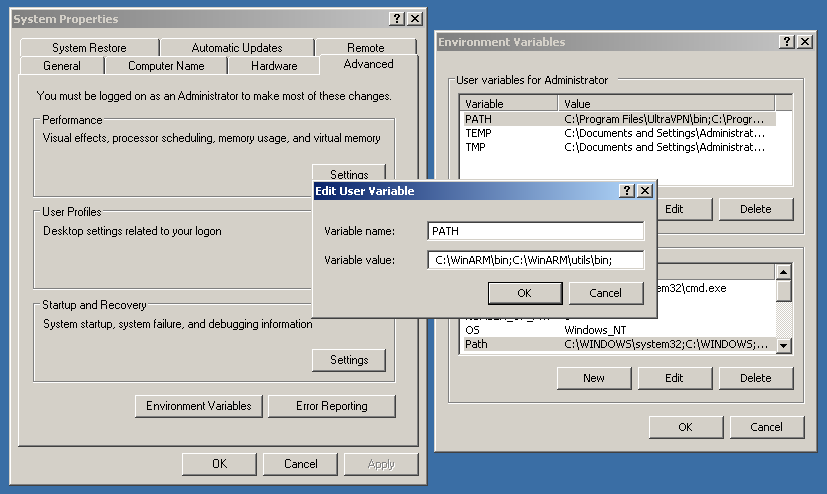
\includegraphics[width=0.95\textwidth]{../images/ch03/winarm-config-win32.png}
 \caption{Konfiguracja narzędzi pakietu WinARM}
 \label{fig:winarm-config}
\end{figure}

\subsection{Instalacja sterowników programatora}
Programowanie oraz debugowanie aplikacji robota może zostać zrealizowane za
pomocą dowolnego programatora kompatybilnego z interfejsem JTAG. Programatory
oparte o interfejs LPT nie wymagają od użytkownika żadnej dodatkowej
konfiguracji. Nieco inaczej wygląda sytuacja z programatorami opartymi o
interfejs USB, które to wymagają przed pierwszym użyciem zainstalowania
sterowników umożliwiających prawidłowe rozpoznanie programatora przez system
Windows. Jednym z bardziej popularnych programatorów USB jest TriTon JTAG. TriTon
JTAG to programator przeznaczony dla procesorów zbudowanych w oparciu o rdzeń ARM
podłączany do komputera za pomocą portu USB. TriTon JTAG posiada standardowe 20
pinowe złącze JTAG wraz z wyprowadzeniami sygnałów RxD i TxD interfejsu UART.
TriTon JTAG współpracuje z OpenOCD, pozwalając na programowanie oraz debugowanie
działającej na urządzeniu aplikacji. Urządzenie oparte jest o układ FT2232 który
umożliwia jego współprace także z innymi środowiskami rozwoju oprogramowania dla
platformy ARM kompatybilnymi z FT2232.

\begin{figure}[h!]
 \centering
 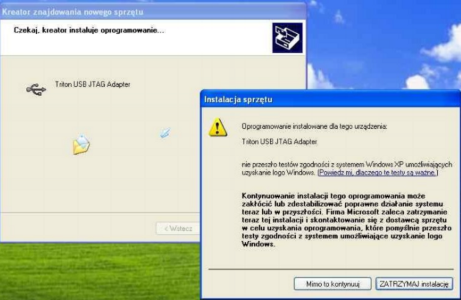
\includegraphics[width=0.85\textwidth]{../images/ch03/jtag-install-s2.png}
 \caption{Instalacja sterowników do programatora TriTon JTAG}
 \label{fig:TritonInstall}
\end{figure}

Instalację programatora należy rozpocząć od pobrania sterowników do układu FT2232
ze strony \url{http://www.ethernut.de/en/download/}. Na stronie dostępne są
sterowniki przeznaczone dla systemów Windows 2000, XP, Server 2003, Vista oraz
Server 2008. Po rozpakowaniu archiwum ze sterownikami należy za pomocą interfejsu
USB podłączyć programator do komputera. Po wykryciu system Windows trzykrotnie
poprosi o podanie ścieżki do sterowników do urządzeń Triton JTAG, Triton USB
RS232 Adapter oraz USB Serial Port. Należy wtedy skazać ścieżkę do katalogu w
którym rozpakowane zostały sterowniki pobrane ze strony wspomnianej wcześniej. Po
poprawnym zakończeniu instalacji w Menadżerze urządzeń systemu Windows widoczne
będą następujące elementy
\begin{itemize}
  \item Triton USB JTAG Adapter,
  \item Triton USB RS232 Adapter,
  \item Triton JTAG
\end{itemize}

\subsection{Instalacja Open On-Chip Debugger}
OpenOCD zostało zapoczątkowane przez Dominika Rath w ramach pracy dyplomowej
realizowanej na uniwersytecie w Augsburg. Od tamtego czasu OpenOCD bardzo się
rozwinęło i urosło do rozmiarów aktywnego projektu open-sourcowego wspieranego
przez programistów z całego świata. Celem OpenOCD jest dostarczenie
uniwersalnego narzędzia umożliwiającego debugowanie i programowanie systemów
wbudowanych.
 
\begin{figure}[h!]
 \centering
 \subfloat{\label{fig:OpenOCD-A}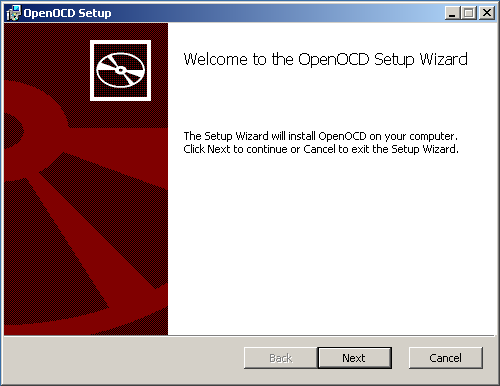
\includegraphics[width=0.7\textwidth]{../images/ch03/open-ocd-install-s1.png}}\hfill
 \subfloat{\label{fig:OpenOCD-B}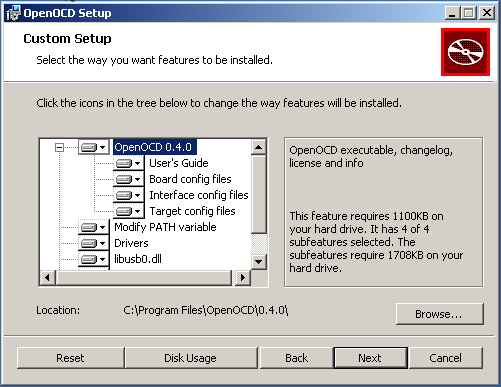
\includegraphics[width=0.7\textwidth]{../images/ch03/open-ocd-install-s2.png}}
 \caption{Instalator Open On-Chip Debugger'a (OpenOCD)}
 \label{fig:openocd-win32-install}
\end{figure}

Strona projektu OpenOCD dostępna jest pod adresem
\url{http://openocd.berlios.de/web/}. Dostępne są tam zarówno źródła jak i
dokumentacja do projektu. Niestety w chwili pisania pracy magisterskiej autorzy
nie udostępniali wersji skompilowanej dla systemu Windows. Dlatego też użyta
została niezależna wersja OpenOCD z przygotowanym instalatorem dla systemu
Windows. Instalator OpenOCD dla Windows jest do pobrania ze strony
\url{http://www.ethernut.de/en/download/}. Po uruchomieniu instalatora wybieramy
lokalizację docelową w której OpenOCD ma zostać zainstalowane. Po zakończeniu
instalacji konieczne jest uzupełnienie wartości zmiennej systemowej PATH ścieżką
do miejsca instalacji OpenOCD, domyślnie \url{C:\ethernut\nut\tools\win32}.

\subsection{Konfiguracja zintegrowanego środowiska programistycznego}
Poprawne zainstalowanie pakietów WinARM oraz OpenOCD dostarcza wszystkich
niezbędnych narzędzi potrzebnych do rozwijania aplikacji dla platform
wbudowanych. Niemniej jednak korzystanie z nich wymaga bezpośredniej interakcji
z linią poleceń systemu Windows, co dla niektórych programistów może być
uciążliwe. Możliwe jest napisanie skryptów systemowych pozwalających na
uruchamianie sekwencji procedur wymaganych np. do zaprogramowania robota,
ale jest to rozwiązanie nieprzenośne i słabo konfigurowalne. Dlatego też zaleca
się instalację zintegrowanego środowiska programistycznego które oprócz edytora
kodu umożliwi automatyzację najczęściej wykonywanych zadań. Wybór rodzaju
środowiska programistycznego zależy niemal w całości od preferencji programisty
gdyż większość potrzebnych narzędzi można bez większych trudności zintegrować z
ulubionym edytorem. Na potrzeby tej pracy omówiona zostanie konfiguracja dla
środowiska Eclipse. Wybór podyktowany został faktem iż jest to obecnie jedna z
najpopularniejszych platform do rozwoju oprogramowania, a co więcej jej
konfiguracja przebiega identycznie dla systemu Windows jak i Linux. Z tego
względu szczegółowy opis procedury konfiguracji zamieszczony został w rozdziale
poświęconym narzędziom dla systemu Linux.

\subsection{Narzędzia dla systemu Linux}
Jednym z wymagań pracy dyplomowej było przygotowanie zestawu narzędzi dla systemu
Linux, dzięki którym będzie możliwy dalszy rozwój robota. Zbiór programów
potrzebnych do rozwoju projektu to: zintegrowane środowisko programistyczne
(IDE), kompilator oraz oprogramowanie pozwalające zaprogramować mikrokontroler.
Bierzący rozdział opisuje sposób instalacji i wykorzystania poszczególnych
narzędzi, a także daje światło na inne tego typu oprogramowanie, które było brane
pod uwagę podczas pracy nad projektem, jednak nie zostało użyte.

\subsubsection{Wybór zintegrowanego środowiska programistycznego}
We wcześniejszej wersji oprogramowanie robota było rozwijane na systemie
Microsoft Windows. Niestety zintegrowane środowisko programistyczne używane do
tej pory nie jest multiplatformowe. Konieczne było zatem dobranie nowego IDE,
które umożliwiało będzie rozwijanie stworzonego wcześniej kodu pod systemem
Linux. Oczywiście biorąc pod uwagę niski budżet projektu, wszelkie płatne
rozwiązania zostały prawie  od razu odrzucone. Rozważaniom zostały poddane
następujące środowiska: Eclipse, Netbeans, CodeWarrior, Kile, ARM Workbench IDE.

\textcolor{red}{TODO: DLACZEGO NIE WYBRALIŚMY INNYCH ??}

Ostatecznie zostało wybrane środowisko Eclipse, które jest dostępne na zasadach
licencji: Eclipse Public License, odpowiadającej wymaganiom projektu.
Najwiekszymi zaletami tego rozwiazania jest łatwość instalacji, konfiguracji oraz
użytkowania. W podjęciu ostatecznej decyzji równie istotne było to, iż
rozwiązania płatne takie jak np. CodeWarrior są bazowane na Eclips'ie. Plusem był
także fakt iż dostępne są różnego rodzaju dodatki do Eclipse'a dedykowane do
rozwoju oprogramowania na mikrokontrolery ARM. Istalacja i sposób wykorzystania
jednego z nich został opisany w \textcolor{red}{ TODO: NUMER DODATKU!!!! },
chociaż nie był on wykorzystywany przez autorów tej pracy.

\subsubsection{Instalacja i konfiguracja Eclipse'a}
Wybrane środowisko programistyczne (Eclipse) jest udostępniane pod adresem:
\url{http://www.eclipse.org/downloads/}. Ściągnięte archiwum rozpakowujemy w
wybranym przez nas miejscu. Przechodzimy następnie do katalogu który został
wydobyty z archiwum i uruchamiamy Eclipse'a.

Oprogramowanie zaraz po pierwszym uruchomieniu zapyta nas o miejsce w którym będą
przechowywane źródła naszego projektu tzw. Workspace. Dobrym pomysłem jest
potwierdzenie ustawień domyślnych i zapamiętanie tej ścieżki.

\begin{figure}
 \centering
 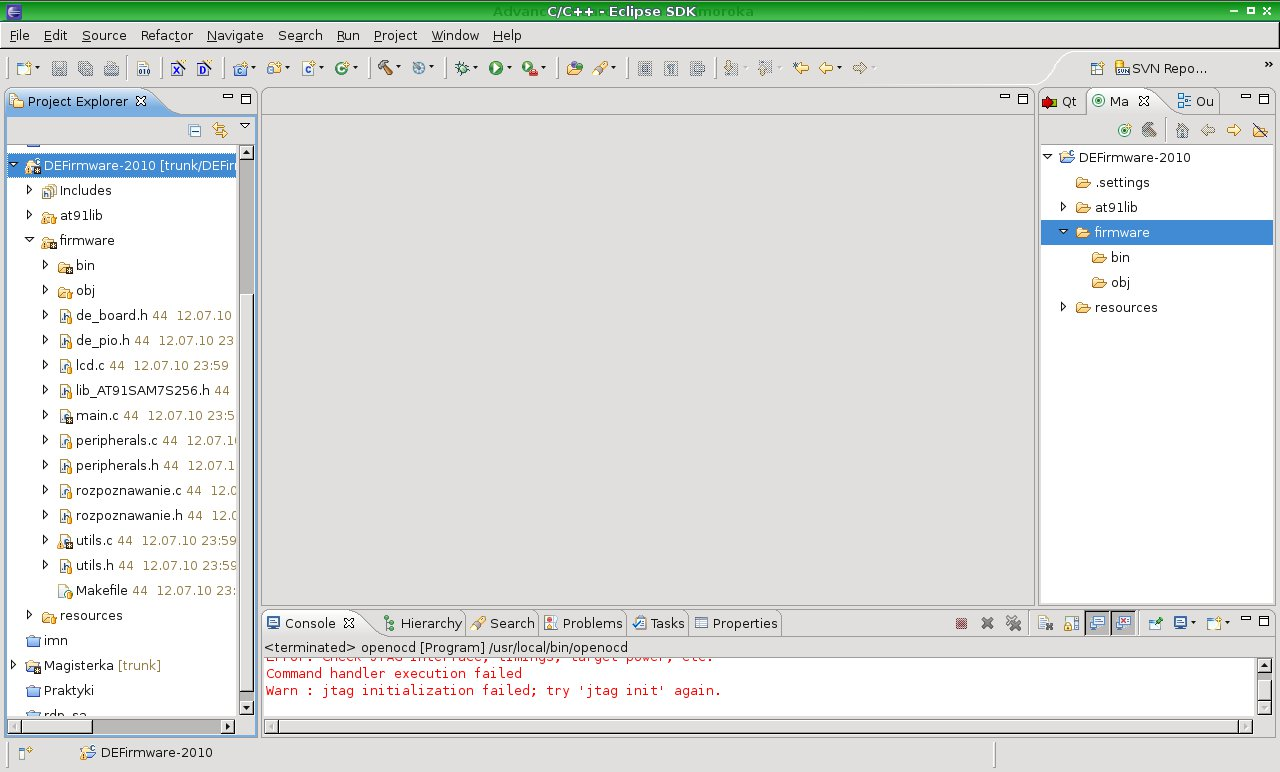
\includegraphics[width=150.0mm]{../images/Eclipse-MainWindow.jpg}
 \caption{Okno główne IDE Eclipse z dodanym projektem}
 \label{fig:Eclipse-MainWindow}
\end{figure}

\paragraph{Dodawanie projektu z firmware'm Dark Explorer'a}
Do workspace'u Eclipse'a należy skopować katalog z kodem sterującym robota.
Następnie dodajemy nowy projekt w IDE wybierając kolejno \textit{File --> New -->
C++ Project}. W oknie dialogowym \textit{C++ Project} (rysunek
\ref{fig:Eclipse-CPP-Project}), należy podać nazwę projektu która powinna być
zgodna z nazwą katalogu zawierającego kod robota. Następnie z listy Project type,
wybieramy \textit{Makefile project --> Empty Project}, a jako \textit{Toolchain}
wybieramy \textit{Other toolchain}. Całą operację zatwierdzamy przyciskiem
\textit{Finish}.

\begin{figure}
 \centering
 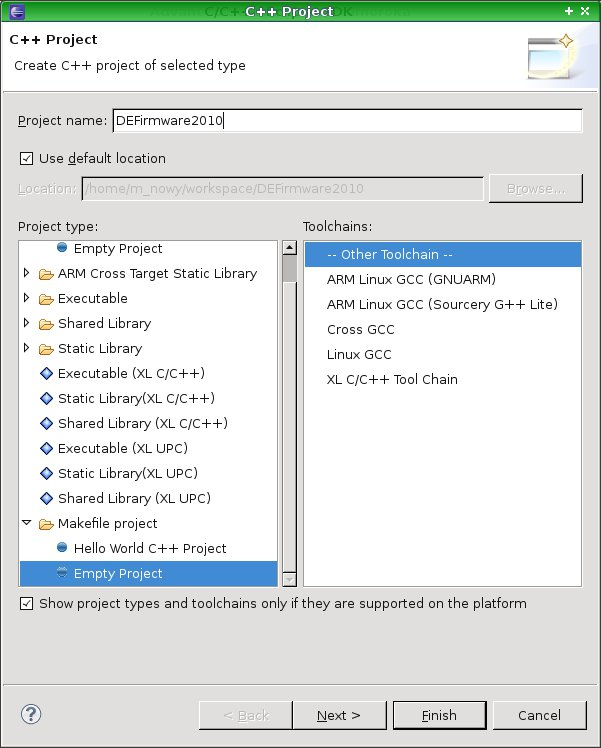
\includegraphics[height=100.0mm]{../images/Eclipse-CPP-Project.jpg}
 \caption{Okno dialogowe C++ Project}
 \label{fig:Eclipse-CPP-Project}
\end{figure}

Po poprawnym dodaniu projektu naszym oczom powinno się ukazać okno podobne do
tego na rysunku \ref{fig:Eclipse-MainWindow}

W przypadku gdy przed uruchomieniem Eclipse'a nie ustawilismy ścieżki do
odpowiedniego toolchain'a w zmiennych środowiskowych systemu. podjąć dodatkowe
kroki. Eclipse umożliwia konfigurowanie tych zmiennych dla pojedyńczych
projektów. W celu ustawienia wymaganej ścieżki klikamy prawym klawiszem myszy na
nazwie naszego projektu w \textit{Project Explorer'ze} i wybieramy
\textit{Properties}.

\begin{figure}
 \centering
 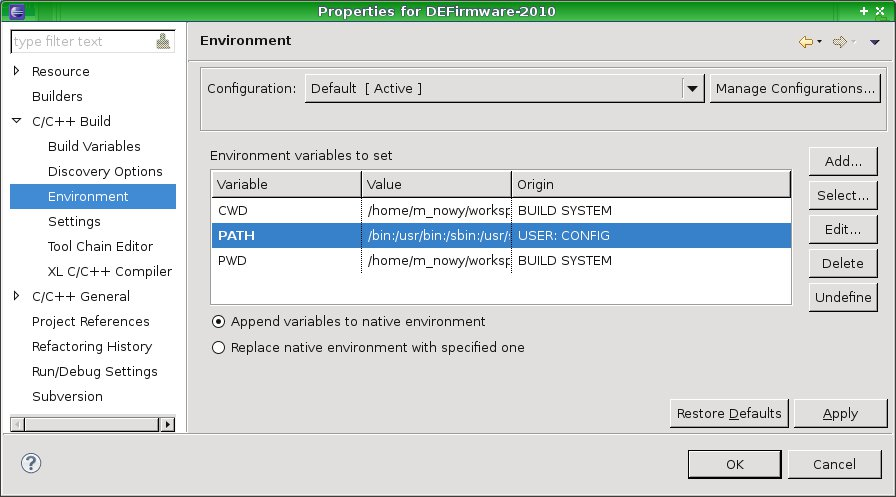
\includegraphics[width=150.0mm]{../images/Eclipse-Project-Properties.jpg}
 \caption{Okno dialogowe Properties}
 \label{fig:Eclipse-Project-Properties}
\end{figure}

Po ukazaniu się okna dialogowego \textit{Properties} (rysunek
\ref{fig:Eclipse-Project-Properties}) wybieramy \textit{C/C++ Build -->
Environment}. Następnie modyfikujemy zmienną \textit{PATH}, dodając na końcu
ścieżkę do naszego toolchain'a.

W celu przetestowania poprawności naszej konfiguracji możemy spróbować
skompilować kod, klikając prawym klawiszem myszy na nazwę projektu, a następnie
wybierając z menu kontekstowego opcję \textit{Build Project}. W wyniku powinniśmy
otrzymać dwa pliki binarne w katalogu \textit{firmware/bin}. Są to pliki gotowe
do umieszczenia w pamięci flash robota.

\subsubsection{Instalacja i konfiguracja toolchain'a}
W celu przetworzenia kodu do formy współpracującej z mikrokontrolerem ARM
niezbędny nam jest odpowiedni toolchain, czyli zestaw narzędzi generujących pliki
wykonywalne oraz pomagających w debugowaniu utworzonego oprogamowania. Tworzony
kod był kompilowany przy pomocy GNUARM toolchain w wersji 3.4.3 dostępnej na
stronie
\url{http://www.gnuarm.com/bu-2.15_gcc-3.4.3-c-c++-java_nl-1.12.0_gi-6.1.tar.bz2}

Po ściągnięciu archiwum ze strony producenta należy rozpakować je do dowolnego
katalogu, na potrzeby tej pracy załóżmy że będzie to katalog \url{/usr/local/} W
celu zapewnienia dostępu do toolchain'a wszystkim programom wskazane jest
dodanie ścieżki /usr/local/bin do zmiennej środowiskowej PATH (komenda 
\verb|export PATH=$PATH:/usr/local/bin|).

W celu sprawdzenia poprawności instalacji należy wykonać komende:
\begin{verbatim}
arm-elf-gcc --version 
\end{verbatim}
której wynikiem powinien być komunikat podobny do tego na rysunku \ref{fig:arm-elf-gcc-test}.

\begin{figure}
 \centering
 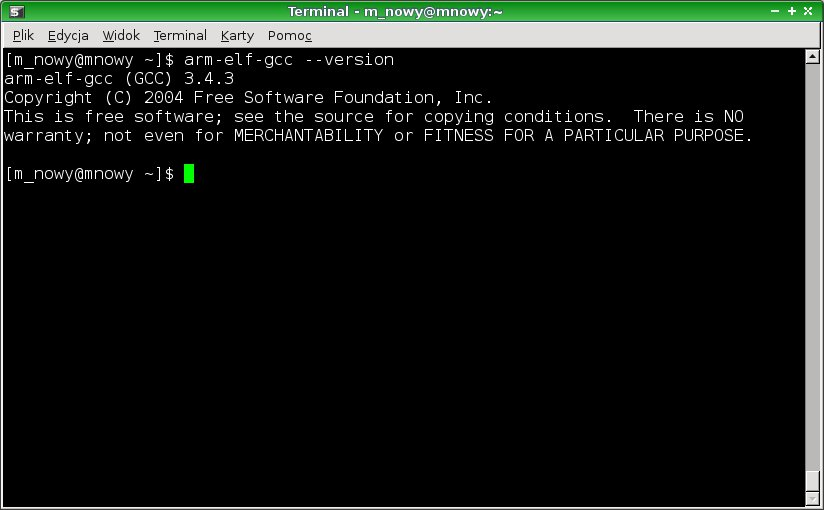
\includegraphics[width=150.0mm]{../images/arm-elf-gcc-test.jpg}
 \caption{Okno pokazujące odpowiedź prawidłowo zainstalowanego kompilatora}
 \label{fig:arm-elf-gcc-test}
\end{figure}

Trzeba wziąć pod uwage to, iż toolchain o którym mowa był przygotowany pod system
32--bit'owy. W przypadku konfiguracji na systemie 64--bit'owym konieczne jest
zaopatrzenie się w 64--bit'ową wersje binarną toolchain'a lub skompilowanie go
samodzielnie. Ewentualne dodatkowe informacje można znaleźć pod adresem
\url{http://www.gnuarm.com}.

\subsubsection{Open On--Chip Debugger -- instalacja i konfiguracja}
\label{roz:opendocd-install}
Pamięć robota była programowana przy pomocy tego samego narzędzia które służy do
sprawdzania poprawności działania napisanego kodu. Mowa tu o oprogramowaniu Open
On--Chip Debugger.

Źródła programu należy pobrać ze strony:
\url{http://sourceforge.net/projects/openocd/}. Autorzy programu nie zamieścili
wersji binarnych, wiec kompilacje będziemy musieli przeprowadzić sami.

Po ściągnieciu i rozpakowaniu źródeł uruchamiamy skrypt configure z odpowiednimi
argumentem'ami przy pomocy komendy:

\begin{verbatim}
./configure --prefix=/usr/local --enable-ft2232_libftdi 
\end{verbatim}

Dodatkowy argument powoduje włączenie obsługi urządzeń bazujących na układzie
FT2232 urzywając biblioteki libftdi. Jest to niezbędne przy korzystaniu z
programatora Triton JTAG A. W przypadku wykorzystywania programatora innej firmy
możliwa będzie konieczność wprowadzenia innego argumentu do skryptu
konfiguracyjnego. Argument prefix określa ścieżke docelową instalacji
oprogramowania.

Gdy skrypt konfiguracyjny zakończy działanie z powodzeniem, możemy wywołać
komende \verb|make && make install| w celu kompilacji i instalacji
oprogramowania.

Po zakończeniu powyższych czynności należy skopiować plik (\textcolor{red}{TODO:
triton.cfg Czy trzeba podawać dokładną ścieżke? płyta? www?}) konfigurujący
połączenie przy pomocy programatora Triton JTAG A do katalogu
\url{/usr/local/openocd/interface}.

W celu przetestowania działania Open On--Chip Debugger'a należy podłączyć
programator Triton JTAG A do portu usb komputera oraz portu JTAG robota. Po
upewnieniu się że robot jest włączony wykonujemy komende:

\begin{verbatim}
openocd -s /usr/local/share/openocd/scripts -f board/atmel_at91sam7s-ek.cfg
-f interface/triton.cfg 
\end{verbatim}

\begin{figure}
 \centering
 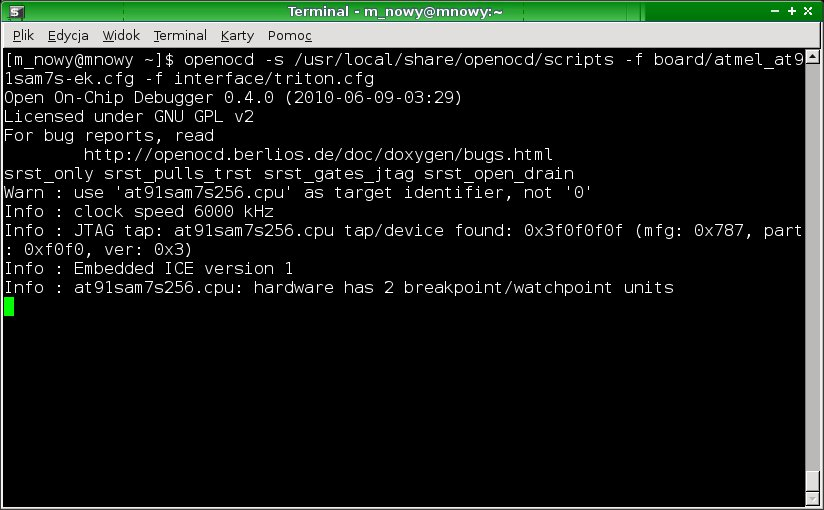
\includegraphics[width=150.0mm]{../images/openocd.jpg}
 \caption{Poprawnie uruchomiony openocd}
 \label{fig:openocd}
\end{figure}

\paragraph{Programowanie pamięci Dark Explorer'a}
W celu wgrania programu do pamięci robota musimy uruchomić dwa narzędzia: telnet
oraz openocd. Procedura instalacji i uruchamiania openocd została opisana
wczesniej w rozdziale \ref{roz:opendocd-install}. W pierwszym kroku uruchamiamy
openocd w celu podłączenia się do robota. Następnie startujemy telnet za pomocą
polecenia:

\begin{verbatim}
 telnet localhost 4444
\end{verbatim}

Zapewnia nam to możliwość wysyłania komend sterujących do openocd. W celu
zaprogramowania pamięci flash Dark Explorer'a i uruchomienia nowej wersji
firmware'u należy wykonać zestaw komend:

\begin{verbatim}
 halt
 flash write_image {ścieżka_do_pliku_elf}
 reset init
 resume
\end{verbatim}

Natomiast w przypadku programowania pamięci RAM robota wykonujemy następujący
zestaw poleceń:

\begin{verbatim}
 halt
 load_image {ścieżka_do_pliku_bin} {początkowy_adres_pamięci}
 reset init
 resume
\end{verbatim}
\section{Platforma mobilna (Windows Mobile 6.1)}
\label{sec:wm-app}
Mobilne urządzenia przenośne z dnia na dzień zyskują na popularności. Każdego
dnia spotykamy się z nimi w domu, w pracy czy spacerując po parku. Z całą
pewnością można stwierdzić, iż większa część społeczeństwa obecnie jest w
posiadaniu telefonu komórkowego, komputera przenośnego czy też jakiegoś innego
urządzenia mobilnego. Wszystkie z wspomnianych urządzeń posiadają
charakterystyczną dla siebie platformę software'ową. Do najlepiej znanych we
współczesnym świecie zaliczyć można między innymi: Windows Mobile, iPhone,
BlackBerry, Symbian OS, Android, Maemo, OpenMoko itp. Każda z wymienionych
platform posiada inną genezę jak również ma swoje mocne i~słabe strony.

Platformy takie jak Windows Mobile, BlackBerry czy iPhone ograniczone
są~do~urządzeń dedykowanych docelowo do współpracy z wspomnianymi środowiskami.
Obok różnorakich problemów z jakimi zmagają się wspomniane wcześniej platformy do
jednego z najpoważniejszych zaliczyć można bardzo ograniczone w niektórych
aspektach API\footnote{Application Programming Interface - interfejs
programowania aplikacji, specyfikacja instrukcji pozwalających na dostęp do
zasobów dostarczanych przez zewnętrzny program}. Nawet tak przenośna platforma
jak Java na urządzeniach przenośnych nie zawsze się sprawdza ze~względu na liczne
braki oraz różnice w~API zmuszające programistów do~tworzenia kodu dedykowanego
dla konkretnego urządzenia. Symbian oraz Windows Mobile wypadają na~tym tle nieco
lepiej ponieważ wspierają szerszą gamę urządzeń jak również ich~API daje więcej
możliwości niż ma to miejsce na przykład w przypadku Javy. Głównym powodem
takiego stanu rzeczy jest bardzo szeroki i różnorodny asortyment platform
sprzętowych utrudniający stworzenie jednolitej i w pełni wykorzystującej
wszystkie możliwości urządzenia platformy programistycznej. Dostępne w chwili
obecnej OpenSource'owe i wieloplatformowe rozwiązania znajdują się ciągle we
wczesnej fazie rozwoju i nie są jeszcze powszechnie znane przez środowiska
twórców oprogramowania.

Firma Microsoft wypuściła po raz pierwszy na światło dzienne swoją platformę
mobilną w latach 90-tych\cite{blog:wm-app-dev}. Natomiast w roku 2002 pojawiła
się pierwsza platforma Windows CE.NET. Zapoczątkowało to popularyzację urządzeń
Pocket PC opartych o system Windows CE 3.0 oraz późniejsze wersje. Dalszy rozwój
bezprzewodowych technologii telekomunikacyjnych pozwolił na integrację telefonu z
komputerem osobistym. Wspomniane urządzenia Pocket PC z 2002 roku wspierały
między innymi standard GSM\footnote{Global System for Mobile Communication,
pierwotnie Groupe Special Mobile - najpopularniejszy obecnie standard telefonii
komórkowej}, GPRS\footnote{General Packet Radio Service - technologia pakietowego
przesyłania danych popularnie stosowana w sieciach GSM}, bluetooth oraz
umożliwiały użytkownikom dostęp do sieci bezprzewodowych. 

W między czasie rozwojowi ulegały urządzenia typu SmartPhone które koncepcyjnie były bardzo
zbliżone do Pocket PC jednakże były one bardziej zbliżone do telefonu niż
komputera osobistego. Podstawową różnicą pomiędzy Smartphone i Pocket PC jest
fakt iż urządzenia Pocket PC posiadają ekran dotykowy, a Smartphone wyposażone są
jedynie w przyciski umożliwiające sterowanie urządzeniem. Każde z tych urządzeń
posiadało inny zestaw aplikacji pomocniczych oraz wspierało inne standardy i
technologie.

W chwili obecnej większość urządzeń Pocket PC oraz Smartphone działają w oparciu
o system Windows Mobile 5 oraz Windows Mobile 6. Nowoczesne urządzenia Pocket PC
wyposażone są w procesor o taktowaniu 500-600 MHz oraz 64-128 MB pamięci RAM.
Najnowsze urządzenia z tej grupy wyposażane są w 1 GHz procesor oraz 512 MB
pamięci.

\subsection{Środowisko rozwojowe}
Tworzenie aplikacji działających na urządzeniach pod kontrolą systemu Windows
Mobile jest niemal tak samo proste jak tworzenie zwykłych aplikacji na komputery
stacjonarne. Niemniej jednak do stworzenia w pełni funkcjonalnego środowiska
rozwojowego (rys. \ref{fig:WMDevelopmentEnviroment}) konieczne jest przejście przez klika kroków przygotowawczych
związanych z~instalacją potrzebnych aplikacji narzędziowych.

\begin{figure}[ht!]
 \centering 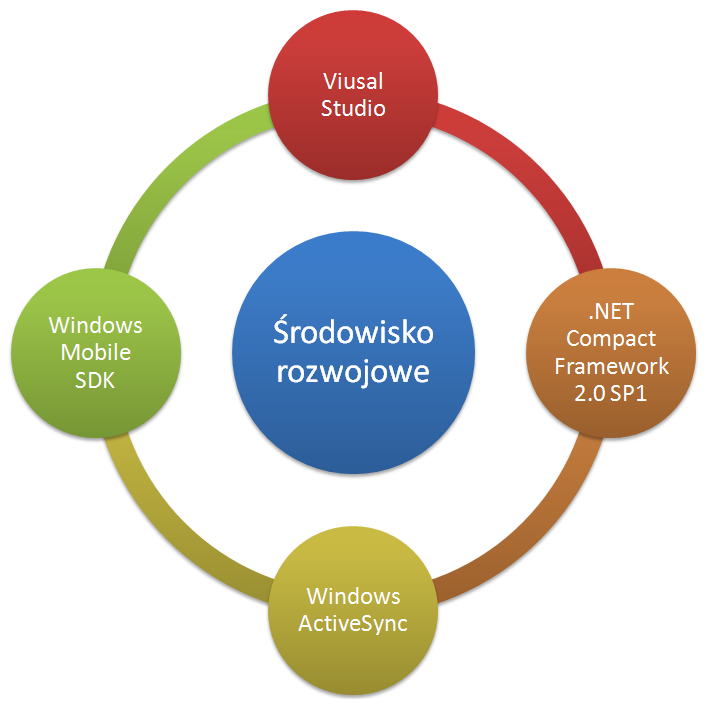
\includegraphics[height=100mm]{../images/ch03/wm_dev_env.png}
 \caption{Elementy składowe środowiska rozwojowego Windows Mobile}
 \label{fig:WMDevelopmentEnviroment}
\end{figure}

Przed rozpoczęciem przygody z tworzeniem aplikacji dla systemu Windows Mobile
konieczne jest zainstalowanie Microsoft Visual Studio. Zaleca się aby Visual
Studio było w wersji 2005 lub 2008. Niestety narzędzia umożliwiające rozwijanie
aplikacji mobilnych nie są poprawnie wykrywane przez Visual Studio 2010 oraz
poprzednie wydania w wersji Express. Dlatego też koniecznością jest instalacja
środowiska w wersji Standard lub~Professional. Każda z tych wersji może zostać
pobrana w wersji czasowej ze stron firmy Microsoft lub w wersji pełnej z
MSDNAA\footnote{Microsoft Developer Network Academic Alliance - program firmy
Microsoft skierowany do studentów i pracowników naukowych w ramach którego
uczestnicy mogą pozyskać darmowe kopie oprogramowania firmy Microsoft}. Visual
Studio posłuży nam nie tylko do edycji kodu aplikacji ale pozwoli również w
prosty sposób budować, debugować oraz przygotować instalator finalnej wersji
aplikacji. Po poprawnym zainstalowaniu środowiska rozwojowego konieczne jest
pobranie i zainstalowanie dostępnych paczek serwisowych dostępnych dla~wybranej
wersji Visual Studio. Pozwoli to uniknąć nieprzyjemnych niespodzianek podczas
instalacji bibliotek narzędziowych i późniejszej pracy.

Jeżeli posiadamy już zainstalowaną kopię Visual Studio możemy przystąpić do
instalacji narzędzi pomocniczych które pomogą nam w tworzeniu aplikacji. Pierwszą
niezbędną biblioteką jest .NET Compact Framework 2.0 SP1. Jest to zestaw narzędzi
wykorzystywanych do uruchamiania aplikacji na platformach opartych o Windows
Mobile. Aby ułatwić sobie proces budowania, debugowania i uruchamiania aplikacji
na urządzeniu konieczne jest zainstalowanie w systemie Windows ActiveSync. Dzięki
ActiveSync możliwe stanie się uruchamianie projektowanej aplikacji, bezpośrednio
z IDE, nie tylko na prawdziwym urządzeniu ale również emulatorze.

Ostatnim, ale i zarazem najważniejszym krokiem jest instalacja Windows Mobile
SDK\footnote{Software Development Kit - zestaw narzędzi programistycznych
niezbędnych do tworzenia aplikacji korzystających z funkcjonalności dostarczonej
przez daną bibliotekę}. Na stronach firmy Microsoft dostępne są dwie wersje SDK,
Standard oraz Professional. Wersja Standard zawiera w sobie tylko wsparcie dla
urządzeń z Windows Mobile Classic lub Standard natomiast wersja Professional
obejmuje wszystkie dostępne środowiska. Wybór SDK można sprowadzić do
następującej zasady. Jeżeli zamierzamy tworzyć oprogramowanie dla urządzeń
Smartphone bez ekranu dotykowego w zupełności wystarczy nam wersja standardowa.
Jeżeli natomiast planujemy napisane aplikacje uruchamiać na PocketPC lub
dotykowych SmartPhone'ach będziemy potrzebować bibliotek systemu Windows Mobile
Classic lub Professional, tak więc konieczne jest użycie SDK w wersji
Professional. Tak jak w przypadku Visual Studio, również tutaj zaleca się
instalację wszystkich dostępnych na stronie producenta aktualizacji i poprawek.
Jest to szczególnie istotne podczas pracy z emulatorami urządzeń. Po
zrealizowaniu tych kroków otrzymujemy w~pełni funkcjonalne środowisko do rozwoju
aplikacji mobilnych dla urządzeń smartphone.

\subsubsection{Modele aplikacji}
Istnieje klika modeli rozwoju aplikacji dla Windows Mobile (rys. \ref{fig:WMDevelopmentModels}), a wybór docelowego
modelu został pozostawiony programiście. Pierwszy z nich służy do tworzenia
aplikacji w kodzie natywnym. Aplikacje pisane zgodnie z tym modelem cechują się
wysoką wydajnością, bezpośrednim dostępem do sprzętu oraz małym zużyciem zasobów.
Do~rozwoju tego rodzaju aplikacji korzysta się z reguły ze środowiska do
rozwijania aplikacji z~użyciem Embeded Visual C++. Główną wadą tego modelu jest
niska przenośność pomiędzy różnymi platformami zwłaszcza jeżeli aplikacja
korzysta z urządzeń specyficznych dla danego modelu urządzenia. Docelowo więc za
pomocą tego modelu tworzy się biblioteki i narzędzia ułatwiające tworzenie
bardziej skomplikowanych aplikacji. Jeżeli więc interesuje nas tworzenie
wysokopoziomowych aplikacji z GUI, skierowanych bezpośrednio do~użytkowników,
zaleca się tworzenie tego typu aplikacji za pomocą kodu zarządzalnego z~użyciem
takich języków jak C\# czy Visual Basic.

\begin{figure}[ht!]
 \centering 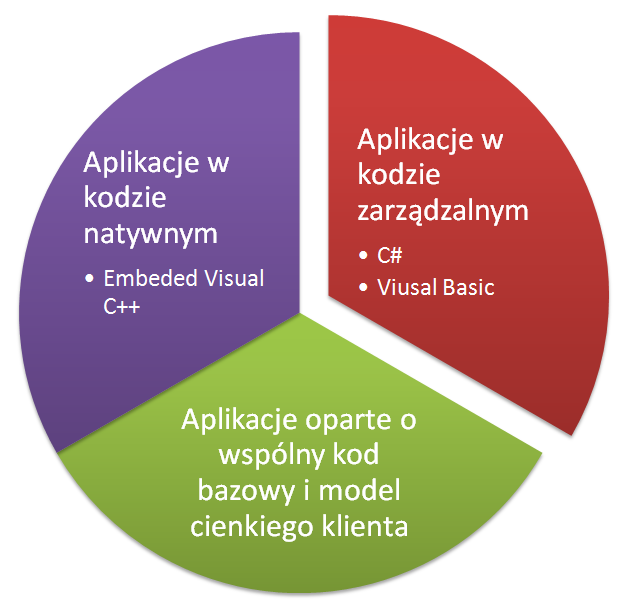
\includegraphics[height=80mm]{../images/ch03/wm_app_models.png}
 \caption{Modele tworzenia aplikacji dla Windows Mobile.}
 \label{fig:WMDevelopmentModels}
\end{figure}

Rozwijanie aplikacji w oparciu o kod zarządzalny pozwala na stworzenie programu
który będzie mógł w pełni wykorzystywać możliwości oferowane przez Microsoft .NET
Compact Framework. Umożliwia to programiście tworzenie rozproszonych systemów
mobilnych pracujących zarówno w modelu ze stałym połączeniem jak i bez. Spora
część narzędzi dostępnych w ramach .NET Compact Framework jest również
wykorzystywana do rozwoju aplikacji na komputery stacjonarne. Biblioteka została
zaprojektowana docelowo na urządzenia o ograniczonych zasobach co w połączeniu z
możliwościami języków z~rodziny .NET oraz integracją z Visual Studio daje nam
profesjonalny zestaw narzędzi do tworzenia aplikacji mobilnych.

Trzecim modelem tworzenia programów pod Windows Mobile jest wykorzystywanie kodu
serwera do pracy z wieloma różnymi typami urządzeń poprzez jeden wspólny kod
bazowy i model cienkiego klienta. Oczywiście tego typu podejście ma sens jedynie
gdy możemy zagwarantować stabilny kanał komunikacyjny pomiędzy urządzeniem
klienta, a~serwerem. Każdy z przedstawionych modeli idealnie sprawdza się jeżeli
tylko w prawidłowy sposób wybierzemy model najbardziej odpowiadający potrzebom
naszej aplikacji.
\subsubsection{Graficzny interfejs użytkownika}
Dzięki wygodnemu systemowi projektowania GUI dostępnego w Visual Studio, tworzenie
interfejsu użytkownika dla platformy mobilnej jest niemal tak proste jak w
przypadku tradycyjnych aplikacji, a jedyną różnicą jest ilość i rodzaj dostępnych
kontrolek. Różnice te wynikają z faktu iż niektóre urządzenia mobilne posiadają
ekrany dotykowe, a~inne nie. Co za tym idzie, rozwój interfejsu użytkownika staje
się bardziej skomplikowany zwłaszcza jeżeli interesuje nas rozwój aplikacji
wspólnej dla obydwu platform sprzętowych. W tym miejscu nie może zabraknąć
informacji, że oprogramowanie zbudowane dla PocketPC nie uruchomi się na
urządzeniach SmartPhone natomiast sytuacja odwrotna jest możliwa do momentu w
którym aplikacja nie zacznie korzystać ze specyficznych funkcji SmartPhone.
Naturalnym stanem rzeczy wydaje się fakt, iż wiele funkcji i komponentów
graficznych znanych z aplikacji desktopowych zostało usunięte z bibliotek Windows
Mobile, aby zapewnić jej wydajność i niewielki rozmiar. Dlatego też pozostawiono
tylko niezbędne, najprostsze komponenty. Ponieważ wydajność  i zasoby pamięciowe
urządzeń stale rosną, również ilość narzędzi dostępnych w SDK jest systematycznie
zwiększana, a~co~za~tym idzie różnice pomiędzy kolejnymi wersjami .NET Compact
Framework są~bardzo duże. Dlatego też posiadanie jak najbardziej aktualnej wersji
SDK ma niebagatelne znaczenie dla wygody tworzenia aplikacji. Podsumowując, rozwój
GUI dla platformy mobilnej nie różni się bardzo od tworzenia interfejsu
użytkownika dla aplikacji dekstopowej. Istnieje również możliwość rozwijania GUI
w oparciu o silniki 3D.W chwili obecnych dostępne są takie rozwiązania jak GAPI
(Game API), OpenGL ES (Embeded Systems), Open VG (Vector Grapics). Jednakże
rozwój takich aplikacji jest niezwykle trudny gdyż wymaga od programisty
tworzenia maksymalnie optymalnego kodu, ze względu na ograniczone możliwości
niektórych urządzeń.

\subsubsection{Komunikacja}
Nowoczesne urządzenia mobilne posiadają szeroką gamę możliwości komunikacyjnych
(rys. \ref{fig:WMCommunicationAPI}). Posiadają one dostęp do szybkich sieci
bezprzewodowych w standardzie 802.11 WiFi. Umożliwiają one również komunikację za pomocą portu podczerwieni, bluetooth czy
USB. Podejmując decyzję na temat wyboru kanału komunikacji należy brać pod uwagę
nie tylko parametry techniczne, ale również liczbę standardów i protokołów
dostępnych dla danego kanału komunikacji. Firma Microsoft dostarcza szereg
interfejsów programistycznych (API) umożliwiających niemal błyskawiczny dostęp do
funkcji komunikacyjnych urządzenia. AcitveSync API dostarcza funkcjonalność
umożliwiającą komunikację za pomocą protokołu synchronizacji. Natomiast Bluetooth
API dostarcza zestaw narzędzi umożliwiających nawiązywanie komunikacji
bezprzewodowej pomiędzy telefonami jak i urządzeniami peryferyjnymi.

\begin{figure}[h!]
 \centering
 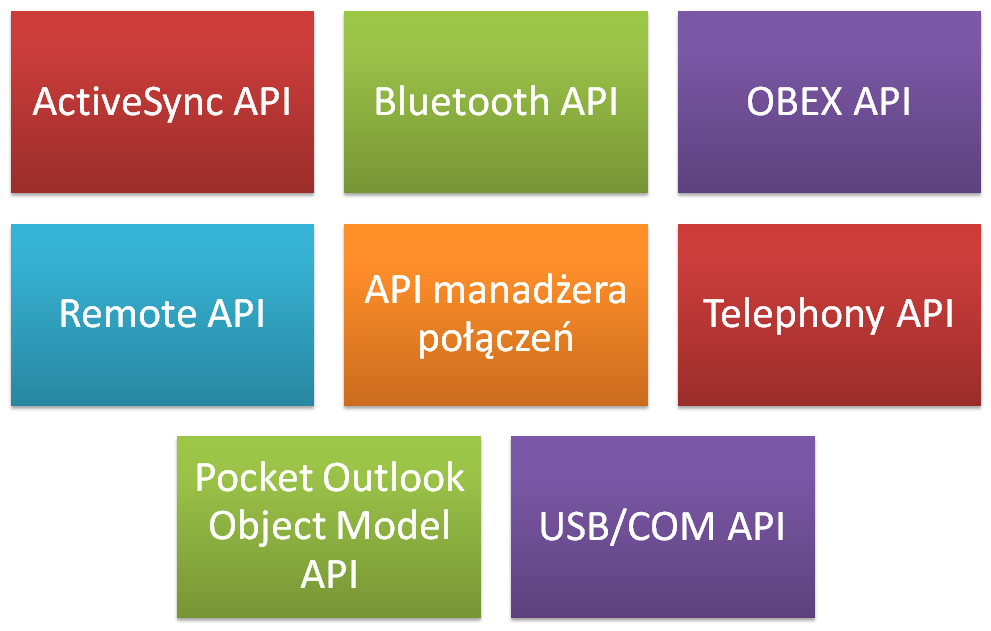
\includegraphics[width=0.9\textwidth]{../images/ch03/wm_comm_api.png}
 \caption{Lista dostępnych na platformie Windows Mobile API komunikacyjnych}
 \label{fig:WMCommunicationAPI}
\end{figure}

API Managera połączeń dostarcza zestaw usług umożliwiających automatyzację
procesu nawiązywania połączenia oraz zarządzanie ich aktywnością. API wymiany
obiektów (OBEX API) dostarcza funkcjonalność umożliwiającą wymianę danych
pomiędzy urządzeniami za pomocą efektywnego, kompaktowego protokołu binarnego
dedykowanego dla urządzeń z ograniczonymi zasobami. Remote API (RAPI) dostarcza
funkcję do zarządzania oraz zdalnego wywoływania metod po stronie urządzenia
klienta. Dostępne są m.in. funkcje dostępu do rejestru, plików, bazy danych czy
też konfiguracji urządzenia. Najważniejszą funkcjonalnością jest jednak możliwość
zdalnego wywoływania procedur. Za pomocą funkcji CeRapiInvoke() przesyłamy do
urządzenia nazwę biblioteki dynamicznej wraz z nazwą metody która ma zostać
wywołana na urządzeniu mobilnym. Kolejnym zestawem narzędzi jest Pocket Outlook
Object Model API. Dostarcza ono funkcje do zarządzania obiektami Pocket Outlook, co
umożliwia synchronizację zadań, kalendarza czy kontaktów za pomocą prostego i
intuicyjnego interfejsu. Dostępne jest również Telephony API (TAPI) które zawiera
w sobie biblioteki umożliwiające zarządzanie kartą SIM oraz wiadomościami SMS.
TAPI udostępnia również zestaw funkcji umożliwiających dostęp do funkcji
telefonowania oraz protokołu WAP. Nie zabrakło również narzędzi do pracy z
portami USB oraz COM. Część z dostępnych portów COM jest zarezerwowana dla
urządzeń wewnętrznych, ale pozostałe dostępne są do pełnej dyspozycji
użytkownika.

\subsubsection{Debugowanie}
Microsoft Visual Studio umożliwia debugowanie aplikacji działających pod kontrolą
Windows Mobile niemal w taki sam sposób jak ma to miejsce w przypadku
tradycyjnych aplikacji desktopowych. Ponadto programista ma do swojej dyspozycji
następujące narzędzia: emulator, panel zarządzania emulowanymi urządzeniami,
panel punktów przerwań i~wątków. Niestety w Visual Studio nie uda się nam
jednocześnie debugować kodu natywnego i zarządzalnego. Możliwe jest natomiast
uruchomienie zarówno projektu napisanego w Visual C++ jak i projektu opartego o
kod zarządzalny, a dzięki funkcjonalności ,,Dołącz do procesu'' możliwe jest
zdalne dołączenie się i monitorowanie procesu działającego na~urządzeniu lub
emulatorze urządzenia. Narzędziem umożliwiającym komunikację pomiędzy urządzeniem
a systemem jest ActiveSync instalowany wraz ze środowiskiem rozwojowym. Za pomocą
narzędzia ActiveSync możemy łączyć się nie tylko z~rzeczywistymi urządzeniami ale
również z emulatorami. Umożliwia to pełną wirtualizację urządzeń mobilnych i
znacznie ułatwia testowanie funkcjonalności zwłaszcza pomiędzy różnymi
platformami urządzeń (SmartPhone, PocketPC). Jedynym ograniczeniem tego procesu
jest możliwość utrzymania tylko jednego aktywnego połączenia co uniemożliwia
debugowanie na wielu urządzeniach jednocześnie. Co więcej, Visual Studio umożliwia
debugowanie jedynie aplikacji stworzonej przez programistę, nie możliwe jest z
poziomu IDE debugowanie aplikacji i usług systemowych działających na urządzeniu.
Do tego typu debugowania konieczne byłoby zbudowanie własnej wersji systemu
Windows Mobile przy użyciu Platform Buildera. Narzędzie to umożliwia również
tworzenie własnego SDK dla Visual Studio i platformy Windows CE. Dodatkową
możliwością dostępną z poziomu emulatora jest emulowanie połączenia z siecią GSM
oraz wsparcie dla GPS. Umożliwia to testowanie, debugowanie i rozwijanie
szerokiego spektrum aplikacji bez konieczności posiadania urządzenia fizycznie.

\subsection{Środowisko uruchomieniowe aplikacji mobilnej}
Docelowym środowiskiem na którym uruchamiana będzie aplikacja sterująca robotem
Dark Explorer będą urządzenia działające pod kontrolą systemu Windows Mobile.
Jedynym wymaganiem stawianym przed urządzeniem na którym podjęta zostanie próba
uruchomienia aplikacji jest posiadanie uprzednio zainstalowanej biblioteki .NET
Compact Framework w wersji co najmniej 2.0 SP1. Wersję instalacyjną biblioteki
dla której były przeprowadzane testy można znaleźć na dołączonej do pracy
płycie. 

\subsubsection{Instalacja aplikacji sterującej}
Przed przystąpieniem do korzystania z mobilnej aplikacji sterującej konieczne
jest jej zainstalowanie na urządzeniu za pomocą którego użytkownik chciałby
komunikować się z robotem mobilnym. Aby tego dokonać konieczne jest skopiowanie
pliku instalatora do pamięci telefonu. Po zakończeniu procesu kopiowania za
pomocą menadżera plików zainstalowanego w telefonie uruchamiamy instalator
aplikacji zgodnie z rysunkiem \ref{fig:wm-install-1}. W przypadku gdy dokonujemy aktualizacji wersji
aplikacji instalator poinformuje użytkownika o wykrytej wersji aplikacji i będzie
wymagał potwierdzenia przed usunięciem poprzedniej wersji i kontynuacją
instalacji obecnej wersji. Komunikat którego może się spodziewać użytkownik
widoczny jest na zdjęciu \ref{fig:wm-install-3}. Kolejnym etapem instalacji
będzie wybór katalogu docelowego w którym zainstalowana zostanie aplikacja
(rys. \ref{fig:wm-install-4}). Po~rozpoczęciu pracy instalator będzie informował
użytkownika o stanie procesu za pomocą widocznego na rysunku
\ref{fig:wm-install-5} paska postępu. Instalacja może zająć od kilku do kilku
dziesięciu sekund w zależności od aktulanego obciążenia i konfiguracji
sprzętowej telefonu. Poprawne zakończenie instalacji zostanie potwierdzone poprzez wyświetlenie
komunikatu widocznego na rysunku \ref{fig:wm-install-6}. Po poprawnym
zainstalowaniu aplikacji konieczne jest jeszcze skonfigurowanie połączenia
bluetooth, aby program sterujący potrafił z niego poprawnie skorzystać. 

W~tym celu należy uruchomić moduł bluetooth zarówno w telefonie jak i robocie.
Następnie należy sparować urządzenia, aby umożliwić im bezpośrednią wymianę
danych bez konieczności potwierdzania przesłania każdego komunikatu. Domyślnym
kodem potrzebnym do nawiązania połącznia bluetooth jest kod ,,0000''. Kolejnym
etapem konfiguracji jest uruchomienie usługi komunikacji za pomocą
protokołu RFCOMM oraz stworzenie nowego portu wychodzącego poprzez który
przesyłane będą dane pomiędzy robotem, a~urządzeniem sterującym. Wszystkie
wspomniane kroki konfiguracyjne zaprezentowane są kolejno na rysunkach
\ref{fig:wm-config-1}, \ref{fig:wm-config-2} oraz \ref{fig:wm-config-3}. Po
zakończeniu tego etapu możliwe jest już rozpoczęcie korzystania z wszystkich
możliwości oferowanych przez aplikację.

 \begin{figure}[h!]
 \centering
 \subfloat[Uruchomienie instalatora]{\label{fig:wm-install-1}
 	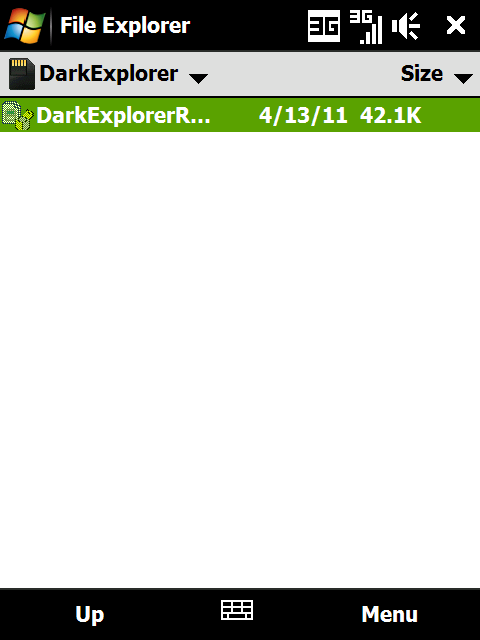
\includegraphics[width=0.30\textwidth]{../images/ch03/wm-install-1.png}}
 \subfloat[Przygotowanie instalacji]{\label{fig:wm-install-2}
 	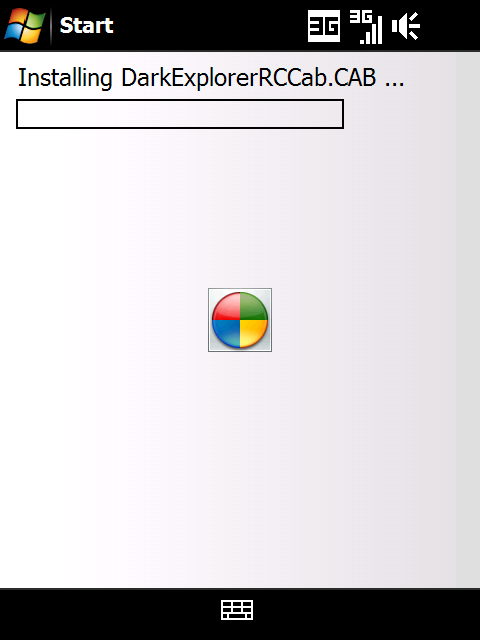
\includegraphics[width=0.30\textwidth]{../images/ch03/wm-install-3.png}}
 \subfloat[Potwierdzanie reinstalacji]{\label{fig:wm-install-3}
 	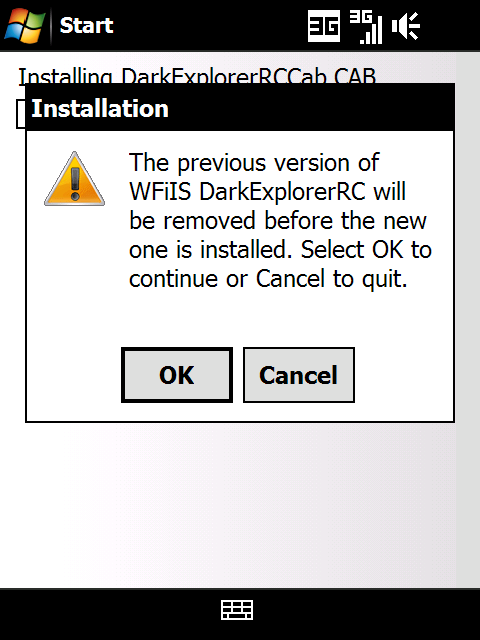
\includegraphics[width=0.30\textwidth]{../images/ch03/wm-install-2.png}} 
 	\hfill \\
 \subfloat[Wybór miejsca instalacji]{\label{fig:wm-install-4}
 	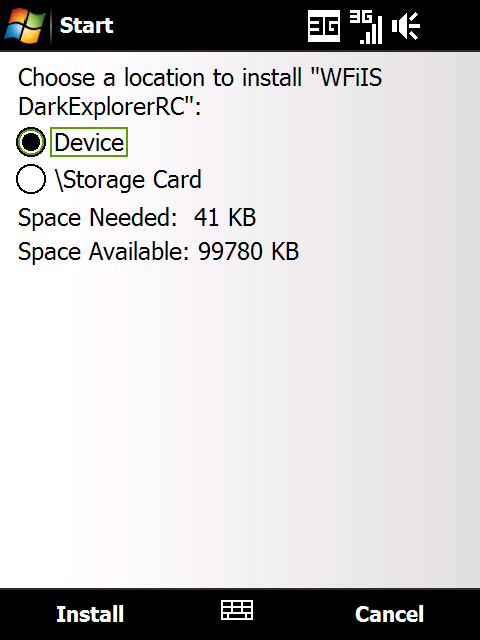
\includegraphics[width=0.30\textwidth]{../images/ch03/wm-install-4.png}}
 \subfloat[Instalator w trakcie działania]{\label{fig:wm-install-5}
 	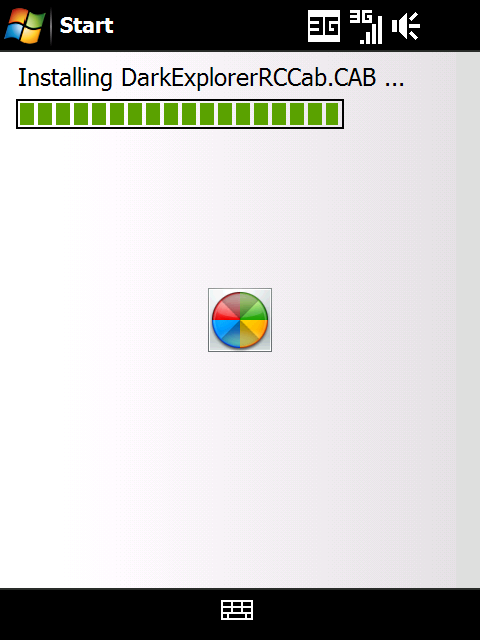
\includegraphics[width=0.30\textwidth]{../images/ch03/wm-install-5.png}}
 \subfloat[Poprawne ukończenie instalacji]{\label{fig:wm-install-6}
 	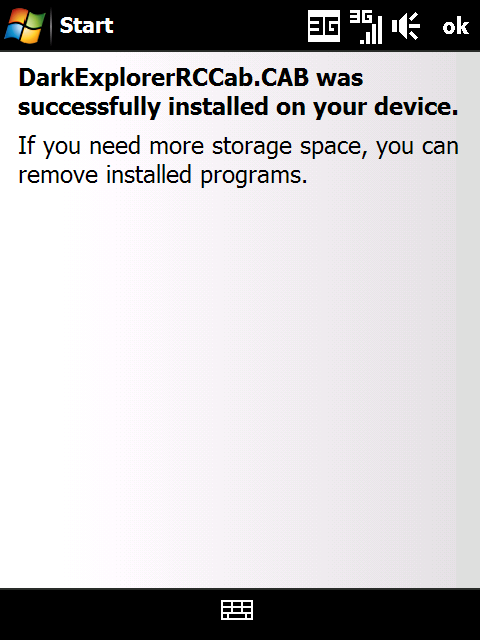
\includegraphics[width=0.30\textwidth]{../images/ch03/wm-install-6.png}}
 		\hfill \\
 \subfloat[Parowanie urządzenia]{\label{fig:wm-config-1}
 	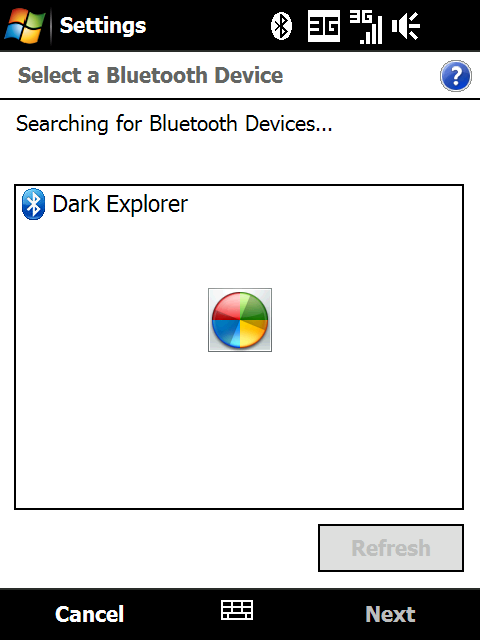
\includegraphics[width=0.30\textwidth]{../images/ch03/wm-config-2.png}}
 \subfloat[Uruchamianie usługi]{\label{fig:wm-config-2}
 	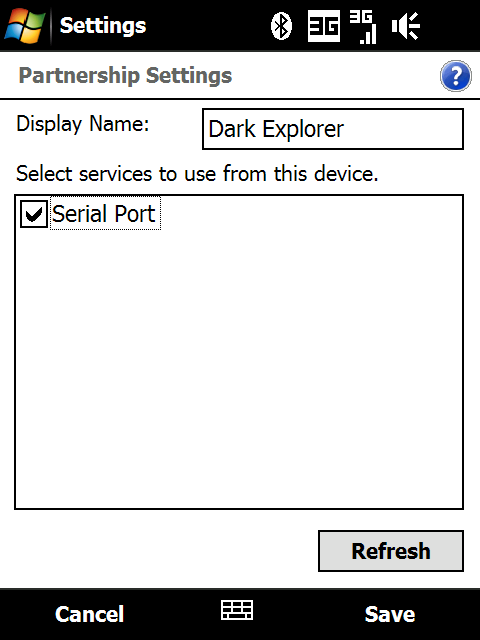
\includegraphics[width=0.30\textwidth]{../images/ch03/wm-config-4.png}}
 \subfloat[Konfiguracja portu COM]{\label{fig:wm-config-3}
 	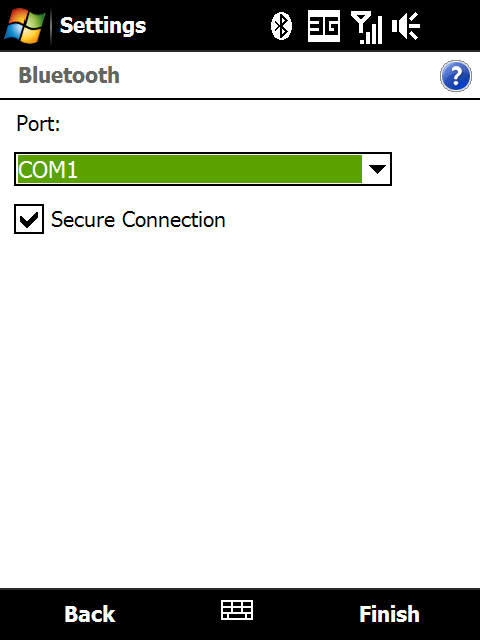
\includegraphics[width=0.30\textwidth]{../images/ch03/wm-config-0.png}}
 \caption{Kroki wymagane do przeprowadzenia poprawnej instalacji i konfiguracji mobilnej aplikacji sterującej}
 \label{fig:wm-install&conf}
\end{figure}
\newpage
\subsubsection{Uruchomienie aplikacji sterującej}
Jeżeli posiadamy już zainstalowaną i skonfigurowaną aplikację sterującą to
możemy rozpocząć korzystanie z jej możliwości. W tym celu należy włączyć robota
i uruchomić moduł bluetooth dostępny w telefonie. Następnie na liście dostępnych
aplikacji należy odszukać program pod nazwą ,,Dark Explorer RC'' ikona programu
widoczna jest na rysunku \ref{fig:wm-app-2}. Wybierając program z listy
zainicjujemy proces jego uruchamiania. Po załadowaniu wszystkich komponentów
aplikacji na ekranie wyświetli się okno główne aplikacji widoczne na rysunku
\ref{fig:wm-app-3}. Aby uprościć dostęp do funkcji programu zostały one
wszystkie zebrane w~menu dostępnym w lewym dolnym rogu aplikacji. Wszystkie
dostępne opcje pogrupowano pod względem tematycznym, tak aby nawet użytkownik
uruchamiający aplikację po~raz pierwszy nie miał trudności z odszukaniem
interesujących go funkcji. 

 \begin{figure}[h!]
 \centering
 \subfloat[Uruchomienie bluetooth]{\label{fig:wm-app-1}
 	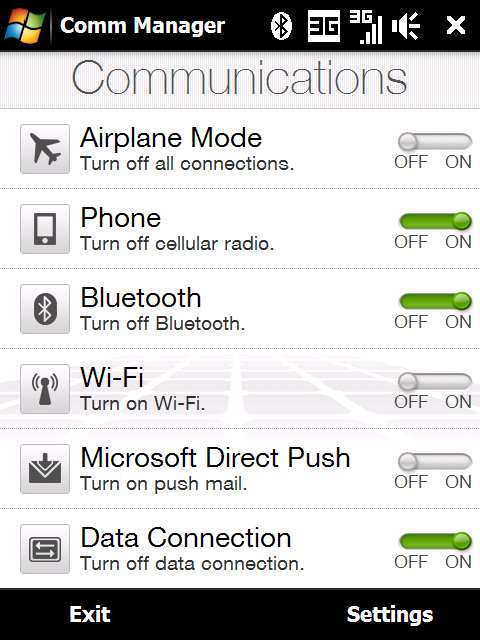
\includegraphics[width=0.30\textwidth]{../images/ch03/wm-app-0.png}}
 \subfloat[Ikona startowa]{\label{fig:wm-app-2}
 	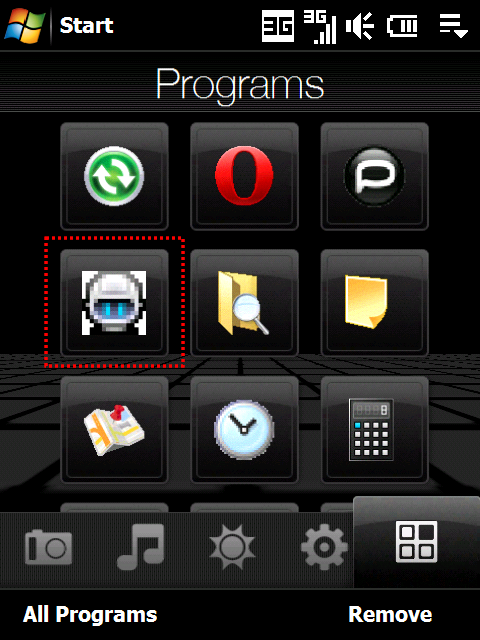
\includegraphics[width=0.30\textwidth]{../images/ch03/wm-app-1.png}}
 \subfloat[Okno główne programu]{\label{fig:wm-app-3}
 	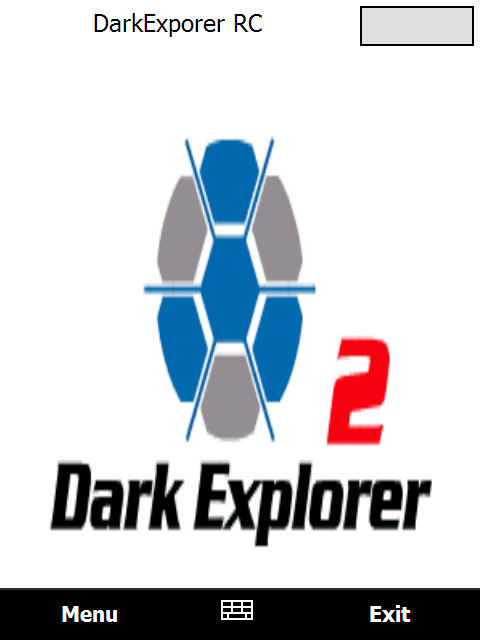
\includegraphics[width=0.30\textwidth]{../images/ch03/wm-app-2.png}} 
 \caption{Uruchomienie mobilnej aplikacji sterującej}
 \label{fig:wm-run}
\end{figure}

Aby uczynić aplikację jeszcze bardziej przyjazną użytkownikowi część funkcji
dostępna jest również pod sprzętowymi przyciskami telefonu. Dobrym przykładem
tego rodzaju funkcji jest sterowanie kierunkiem jazdy robota. Dostęp do tej
funkcjonalności można uzyskać bezpośrednio za pomocą przycisków strzałek
góra, dół, prawo, lewo. Ponad to~naciskając przycisk środkowy użytkownik ma
możliwość pobrania danych z~kamery zgodnie z~aktualną konfiguracją aplikacji.
Dodatkowym atutem programu jest możliwość sterownia kierunkiem jazdy robota za
pomocą akcelerometru jeżeli urządzenie mobilne jest w takowy wyposażone.
Aktualny stan robota oraz aplikacji prezentowany jest w pasku statusu widocznym
u góry okna głównego aplikacji. Pozwala to użytkownikowi na~bieżąco monitorować
nie tylko stan aplikacji ale również to co w chwili obecnej dzieje się na~robocie.

\newpage
\part{Rozwój platformy robota mobilnego}
\section{Lokalizcja twarzy na obrazie}
\subsection{Algorytmy}
\subsection{Implementacja}
\section{Czujniki podczerwieni}
\subsection{Omijanie przeszkód}

\newpage
\part{Podsumowanie}
\section{Testy platformy programowej}
\section{Testy platformy sprzętowej}
\section{Wnioski}

\newpage
\part{Kod źródłowy}

%Cite Test~\cite{website:robotyka-pl}
\newpage

\bibliography{bibliography}{}
\bibliographystyle{plainpl}

\newpage

\end{document}
